\documentclass[12pt]{ctexart}
\usepackage[english]{babel} 
\usepackage{fullpage,mathpazo,amsfonts,nicefrac}
\usepackage{mathtools,amssymb}
\usepackage{float}
\usepackage{hyperref}
\newcommand{\N}{\mathbb{N}}
\newcommand{\Z}{\mathbb{Z}}
\newcommand{\Q}{\mathbb{Q}}
\newcommand{\R}{\mathbb{R}}
\newcommand{\norm}[1]{\left\lVert#1\right\rVert} % norm: double vertical bars

\title{	
\normalfont \normalsize 
\huge PRML Project 1\\ % The assignment title
}

\author{Hao Chen (904547539)} % Your university, school and/or department name(s)

\begin{document}

\maketitle

%\section*{EE236A: Homework 1}
\section{Part 1: ASM and AAM model for face reconstruction.}
\begin{enumerate}
\item

\begin{enumerate}
\item
Using function {\bf{mean}} can calculate the mean face easily. 
\begin{figure}[h!]
  \centering
  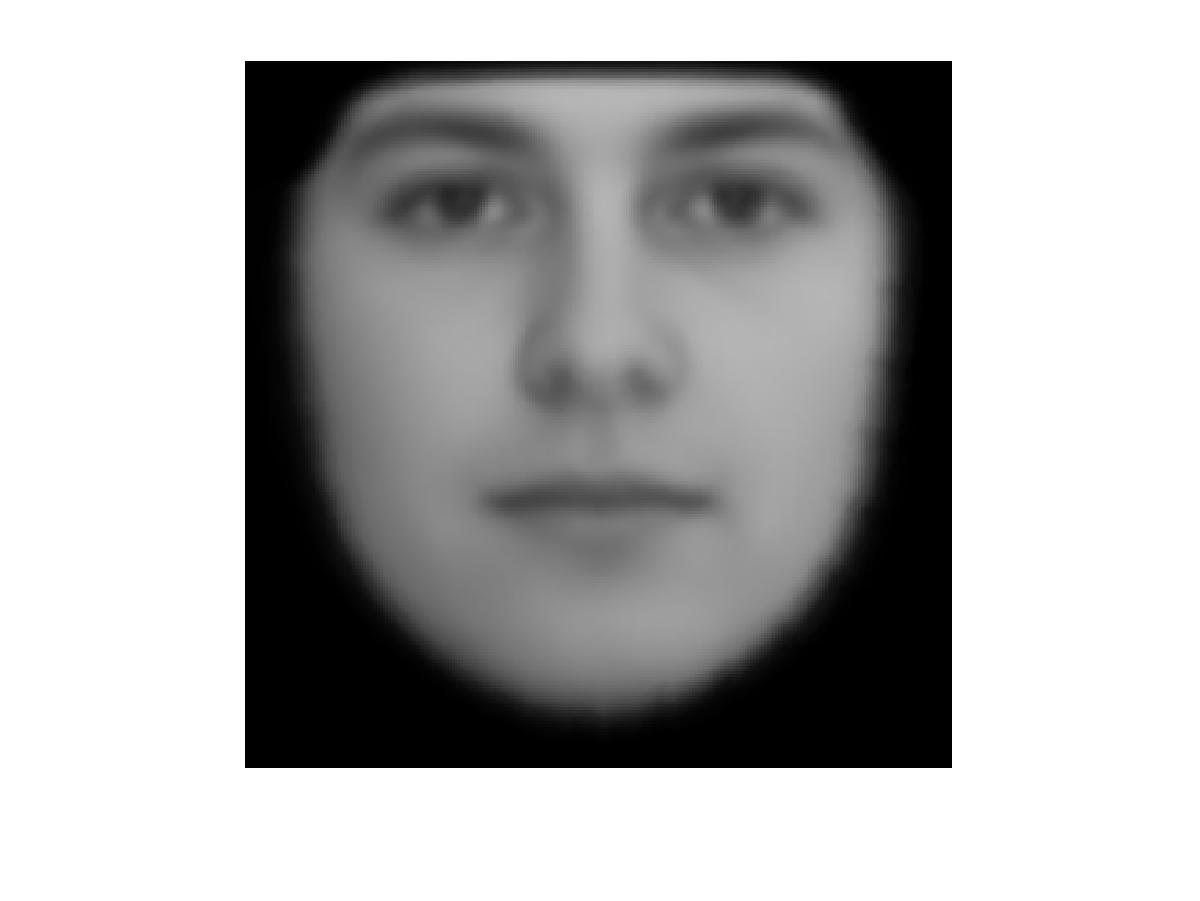
\includegraphics[scale=0.2]{a_mean_face.jpg}
  \caption{mean face}
\end{figure}

\item
We cannot directly use PCA in such high dimension space, where each data is in $256*256$ dimension. However, we are able to calculate the PCA for high-dimensional data where the number of dataset are far smaller than the number of features. Basically, the idea is base on $X'X$ and $XX'$ have same eigenvalues and their eigenvectors can transfer to another's easily. \\
We can resolve PCA as follows. Let X to be the $(N * D)$ dimensional centre data matrix, where each row is a data example. (In our case, $N = 150, D = 256*256$). The scatter matrix is $X'X$. We want to calculate the eigenvalues and corresponding eigenvectors for the scatter matrix. \\
As we can see, if $\lambda_i, u_i$ is one of eigenvalue and corresponding eigenvector of $X'X$,  then $X'X u_i = \lambda_i u_i$. Now pre-multiply both sides by $X$ to give $XX' (Xu_i) = \lambda_i (X u_i)$, which means that $\lambda_i$ is the eigenvalue for $XX'$, and $Xu_i$ is the corresponding vector. It can also see that the eigenvectors of $XX'$ are able to transform to the eigenvectors of $X'X$ in the same way. \\
Thus, we can solve the eigenvector problem in spaces of lower dimensionality instead of spaces of higher dimensionality. Figure.2 shows the first 20 eigen-faces. \\
\begin{figure}[H]
  \centering
  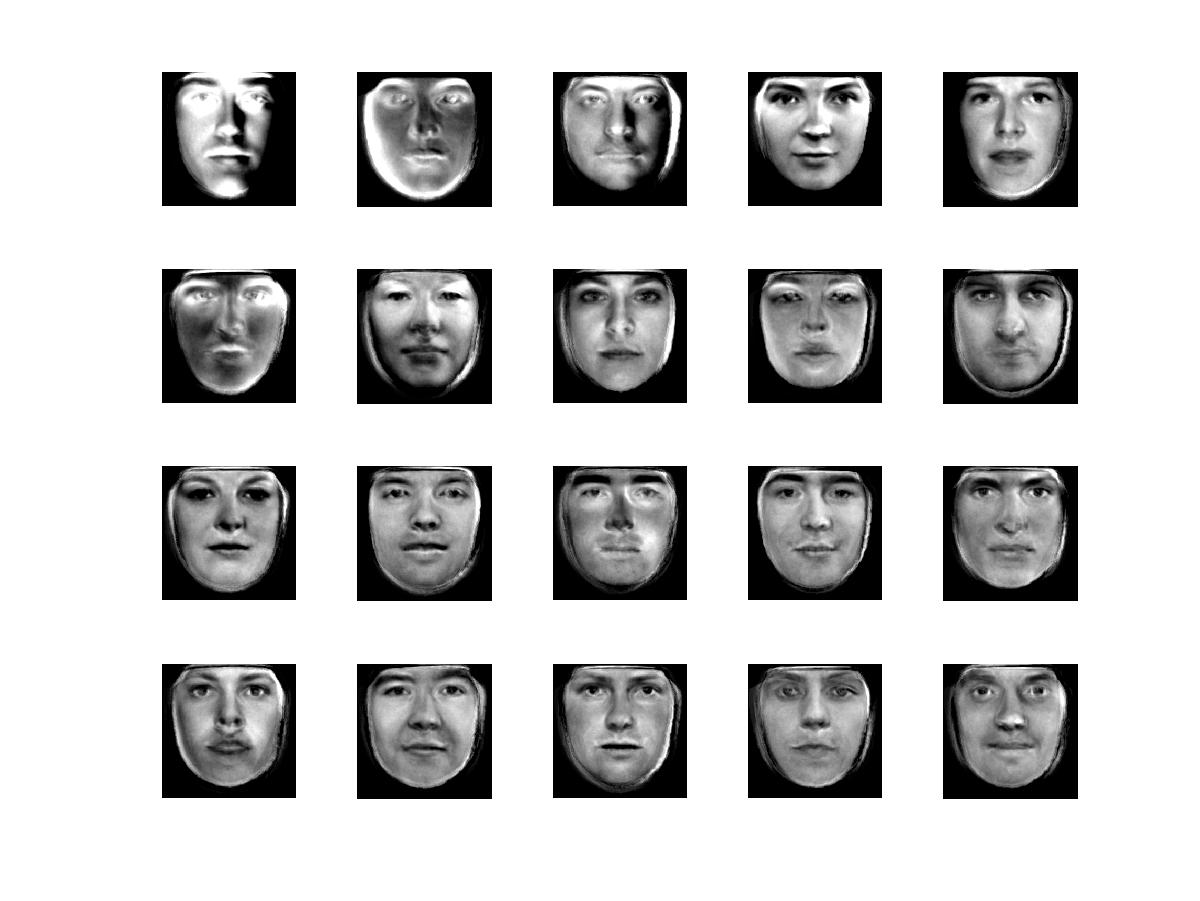
\includegraphics[scale=0.3]{a_first20eigenface.jpg} 
  \caption{First 20 eigen-faces}
\end{figure}

\item 
For each image $x$, we can get the reconstruct face by projecting the face into eigen-faces ($u_1, u_2, ... u_{20}$), which is given by $x_{rec} = \mu + \sum_i <u_i, x> u_i$, where $\mu$ is mean face and $<a, b>$ is inner product. Figure.3 shows the faces which reconstruct by first 20 eigen-faces.  \\
\begin{figure}[H]
  \centering
  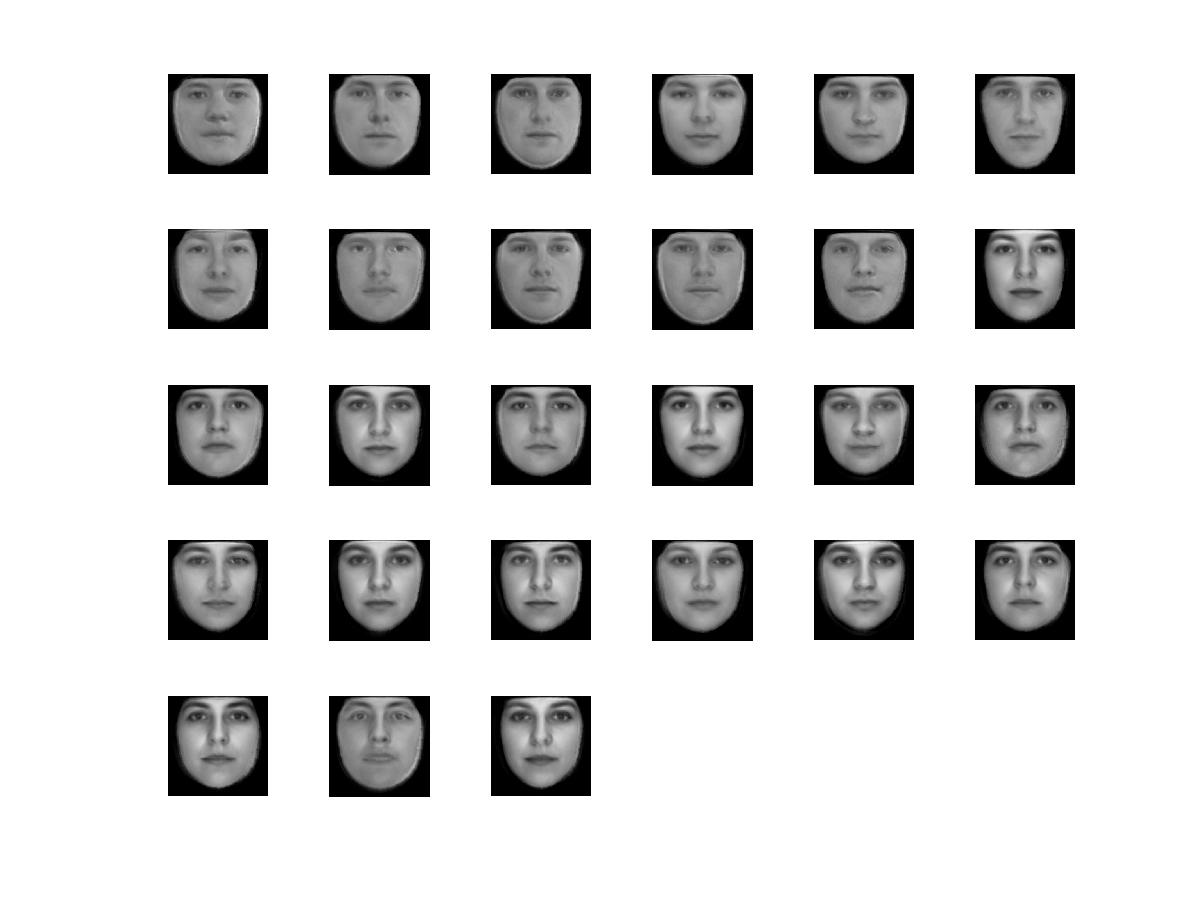
\includegraphics[scale=0.3]{a_reconstrustface.jpg} 
  \caption{Reconstruct faces of test}
\end{figure}

\item
Reconstruct error is define as $e = \frac{1}{|Data|} \sum_{x \in Data} ||x - x_{rec}||^2 / D$, where $D$ is dimension of $x$. We can follow this formula to get the reconstruct error over the number of eigen-faces k. Figure.4 shows the error plot. \\
\begin{figure}[H]
  \centering
  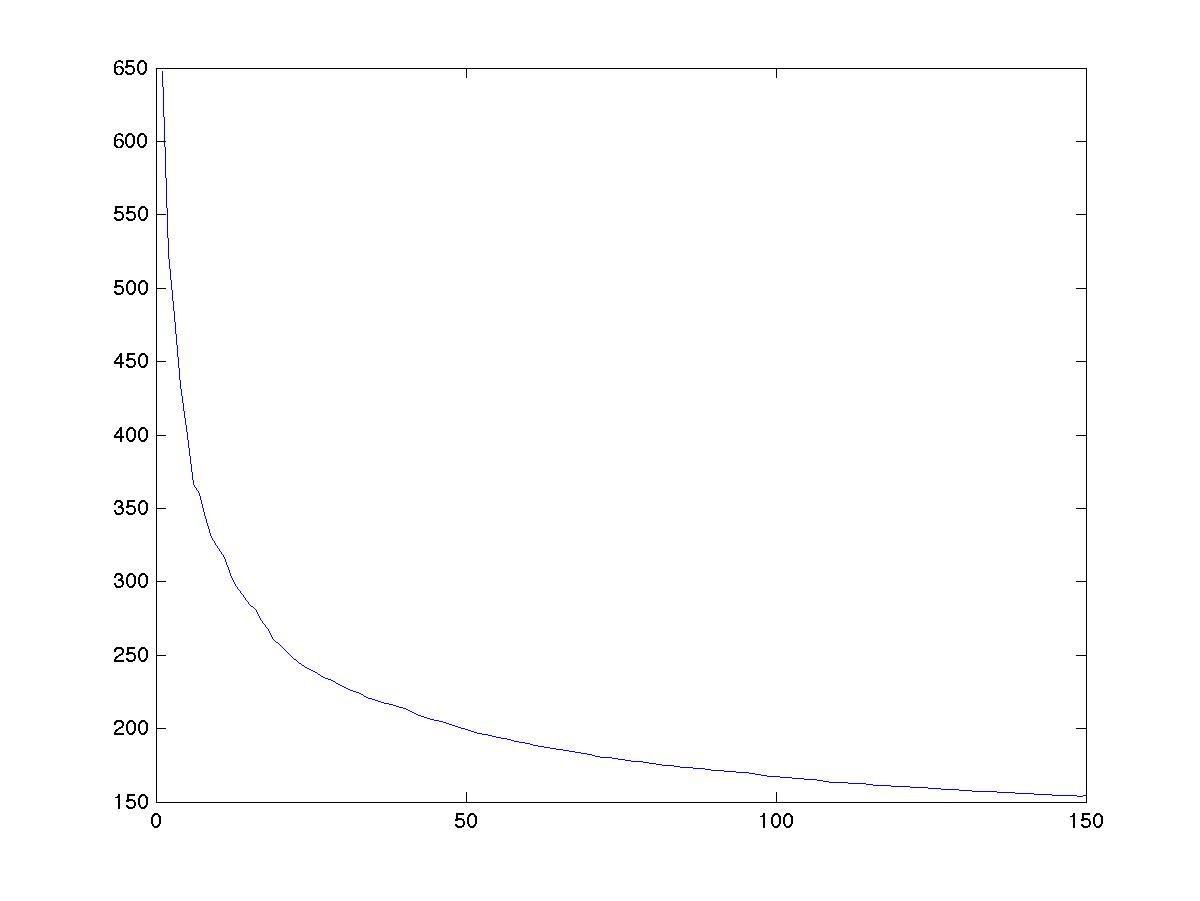
\includegraphics[scale=0.2]{a_reconstructerror.jpg} 
  \caption{Reconstruct Error}
\end{figure} 
\end{enumerate}

\item
All data now are landmark instead of image. However, the k-eigen-warpping of landmarks, reconstruction landmarks, the reconstruction error plot can be get in the same way which mention in (1). We just substitute image data to landmark data. \\ 
Figure.5 shows the mean face with mean landmark. Figure.6 shows the first 5 eigen wrappings.
\begin{figure}[H]
  \centering
  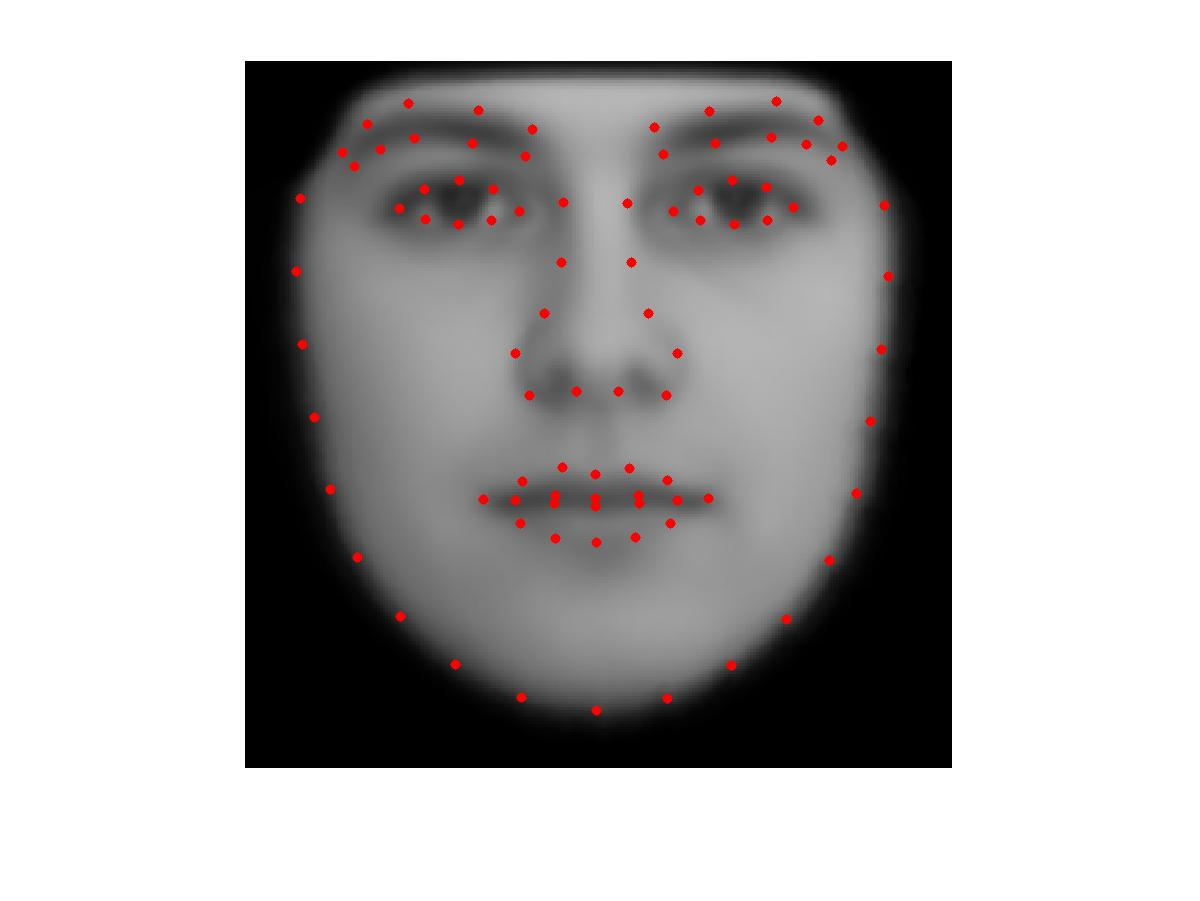
\includegraphics[scale=0.2]{b_mean_lm.jpg} 
  \caption{mean face with mean landmark}
\end{figure}

\begin{figure}[H]
  \centering
  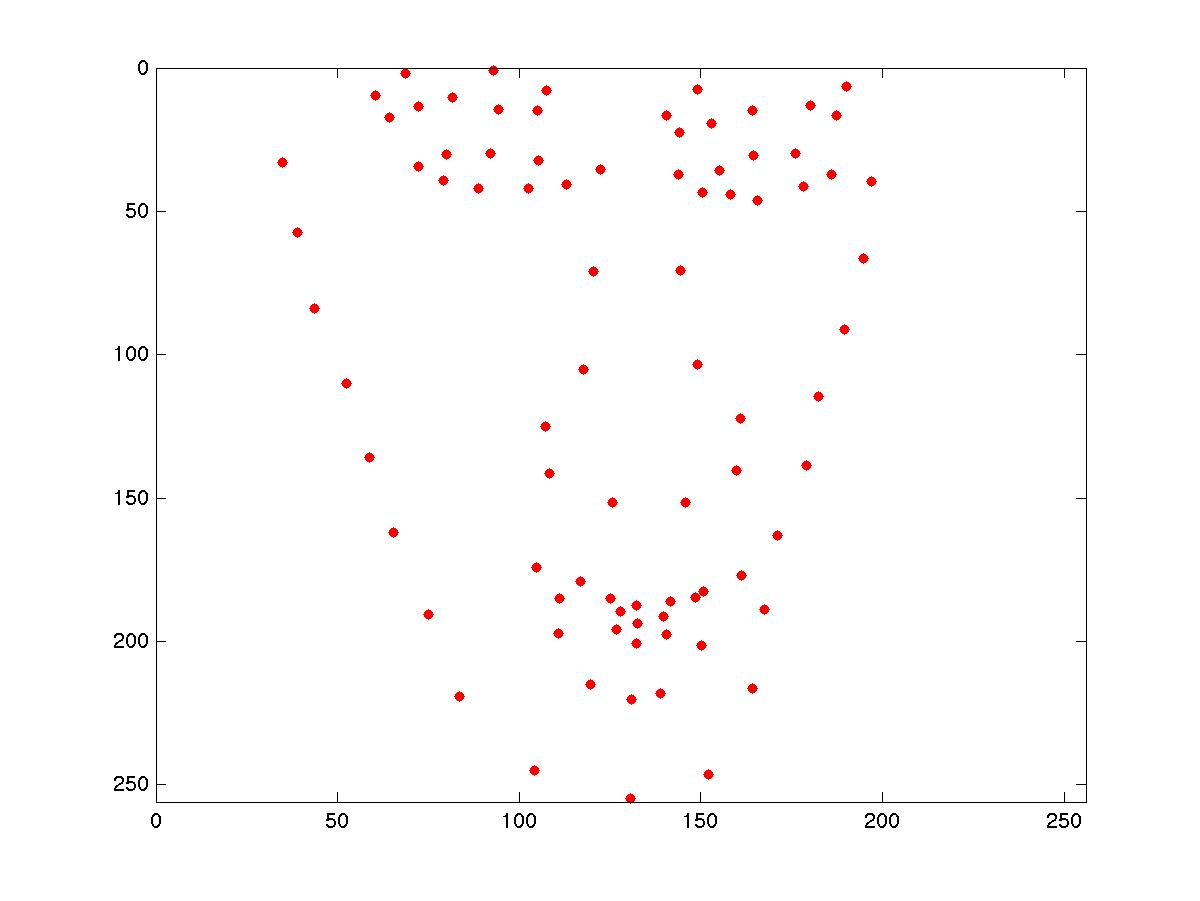
\includegraphics[scale=0.15]{b_eigenlm1.jpg} 
  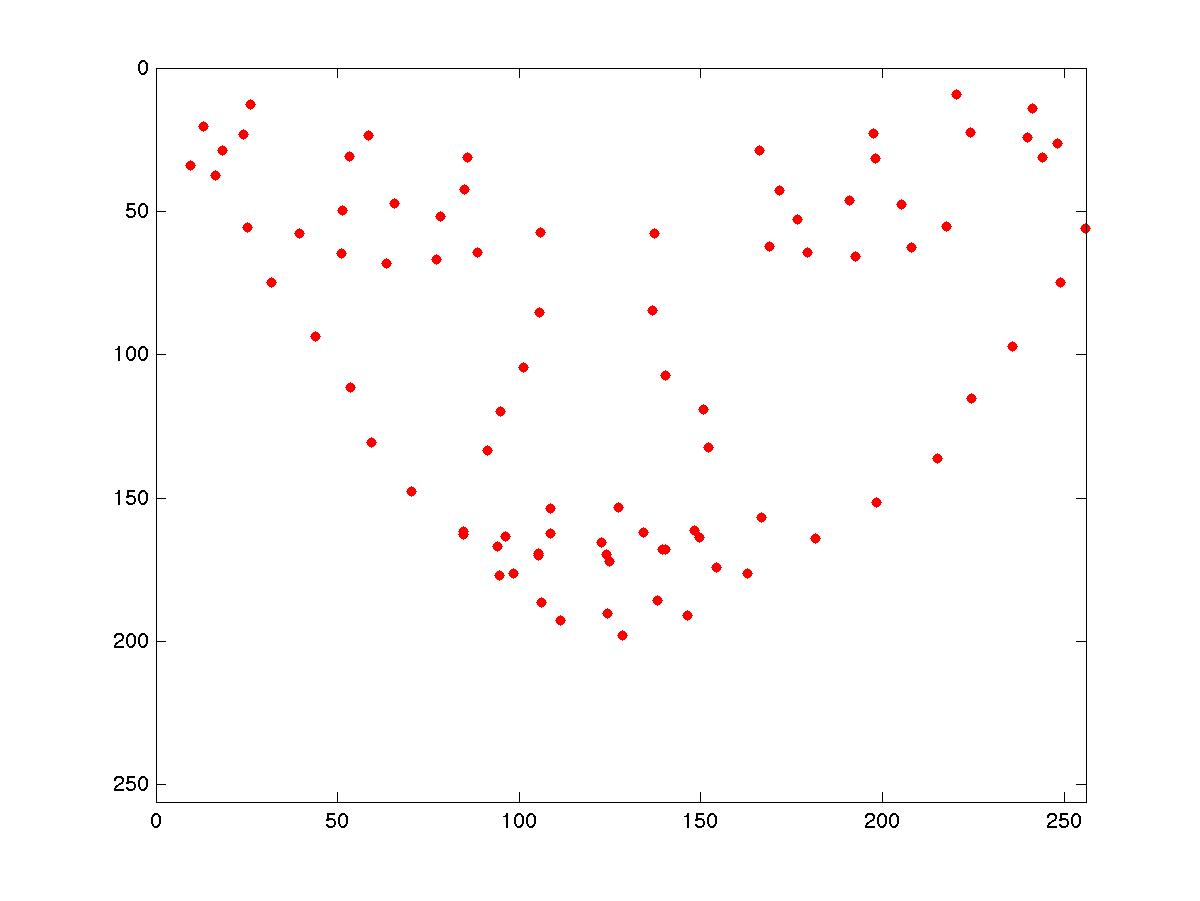
\includegraphics[scale=0.15]{b_eigenlm2.jpg} 
  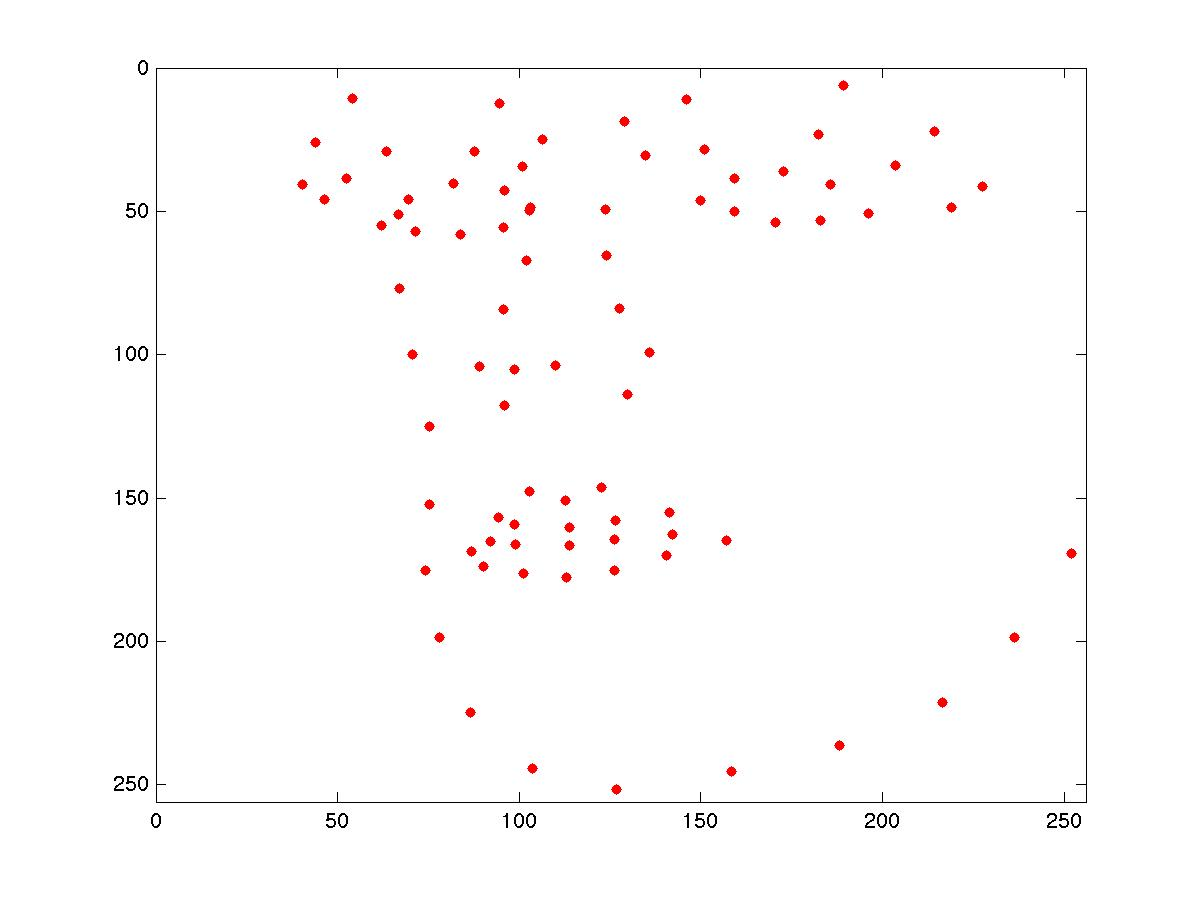
\includegraphics[scale=0.15]{b_eigenlm3.jpg} 
  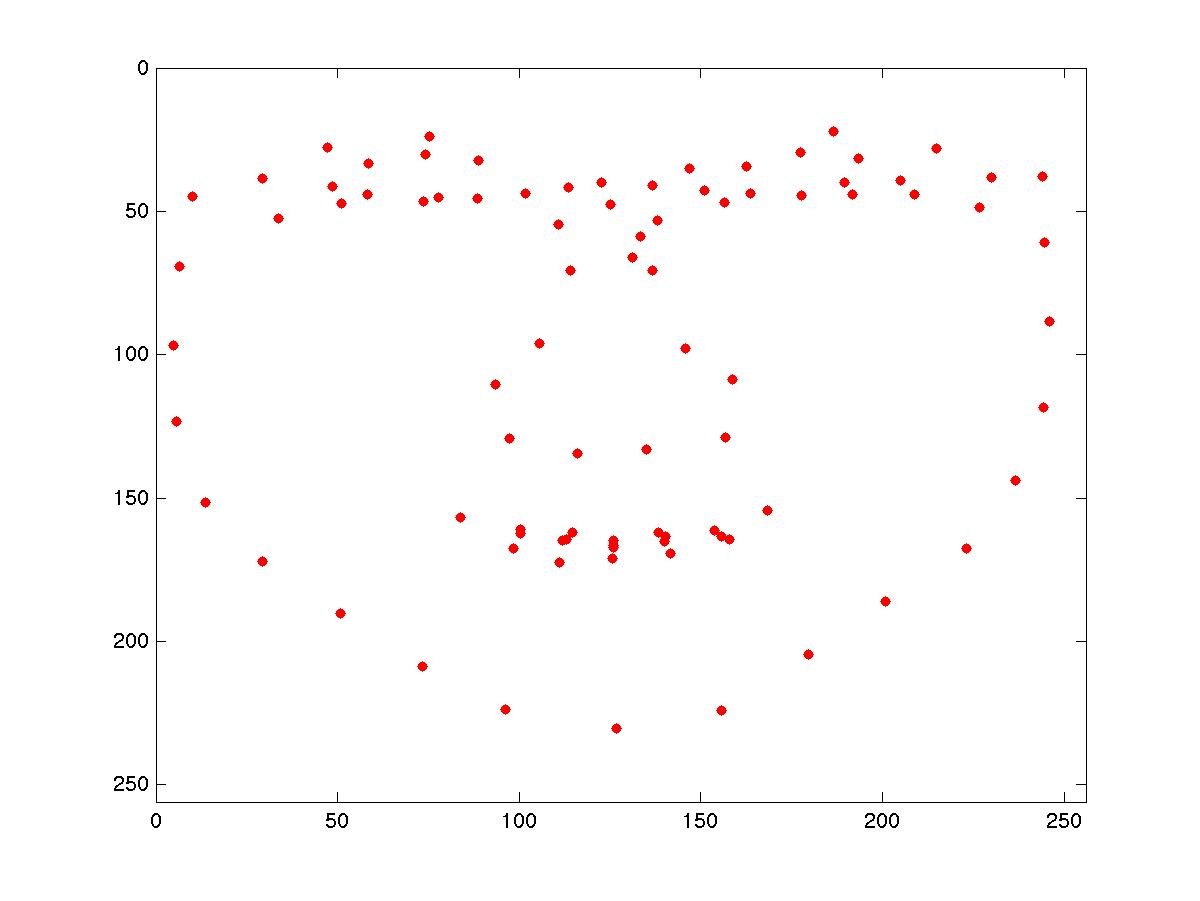
\includegraphics[scale=0.15]{b_eigenlm4.jpg} 
  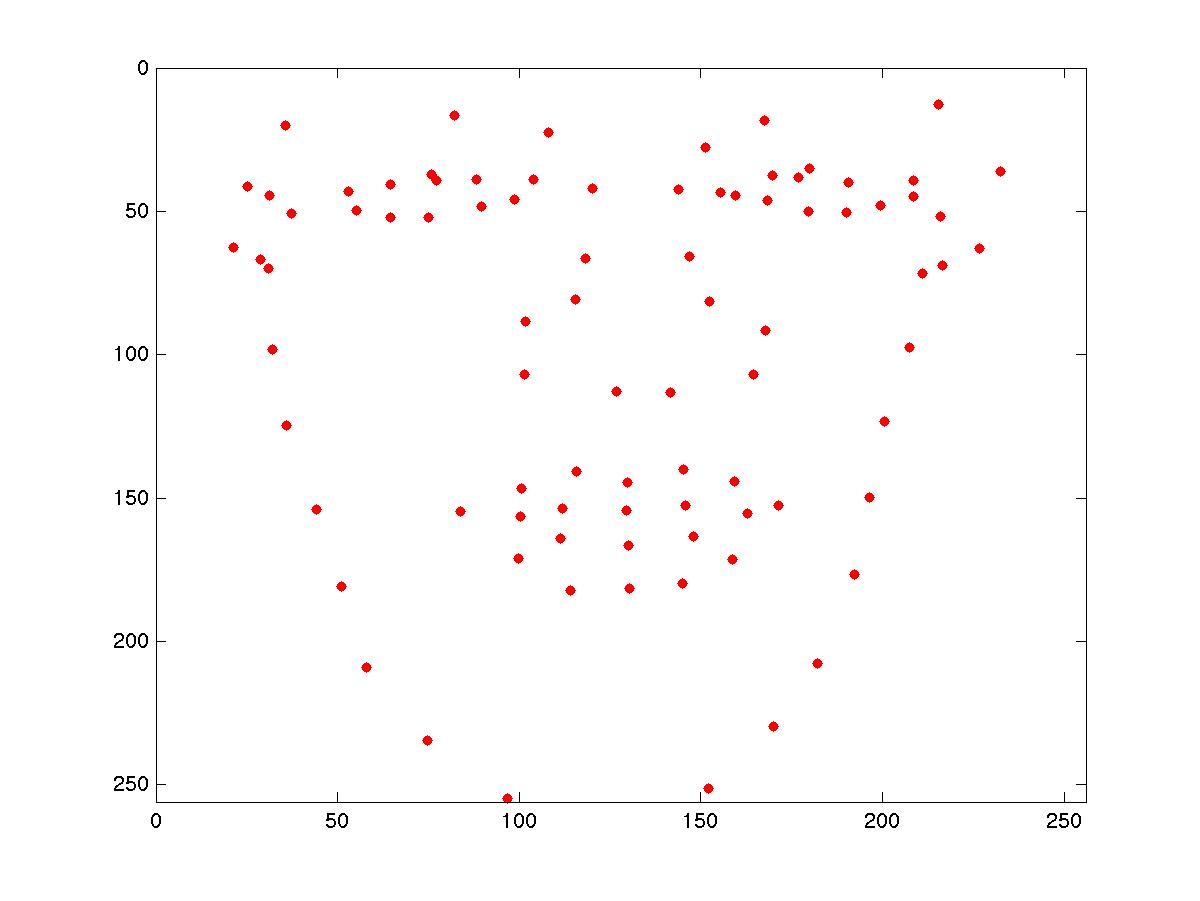
\includegraphics[scale=0.15]{b_eigenlm5.jpg} 
  \caption{first 5 eigen wrappings}
\end{figure}

Figure.7 and Figure.8 show the reconstruction of landmarks for the test faces using first 5 eigen wrapppings. The left side of each pair image is the face with reconstruction landmark, the right side is the face with original landmark. As we can see in the figures, the reconstructions are pretty precise, they only have some small biases.
\begin{figure}[H]
  \centering
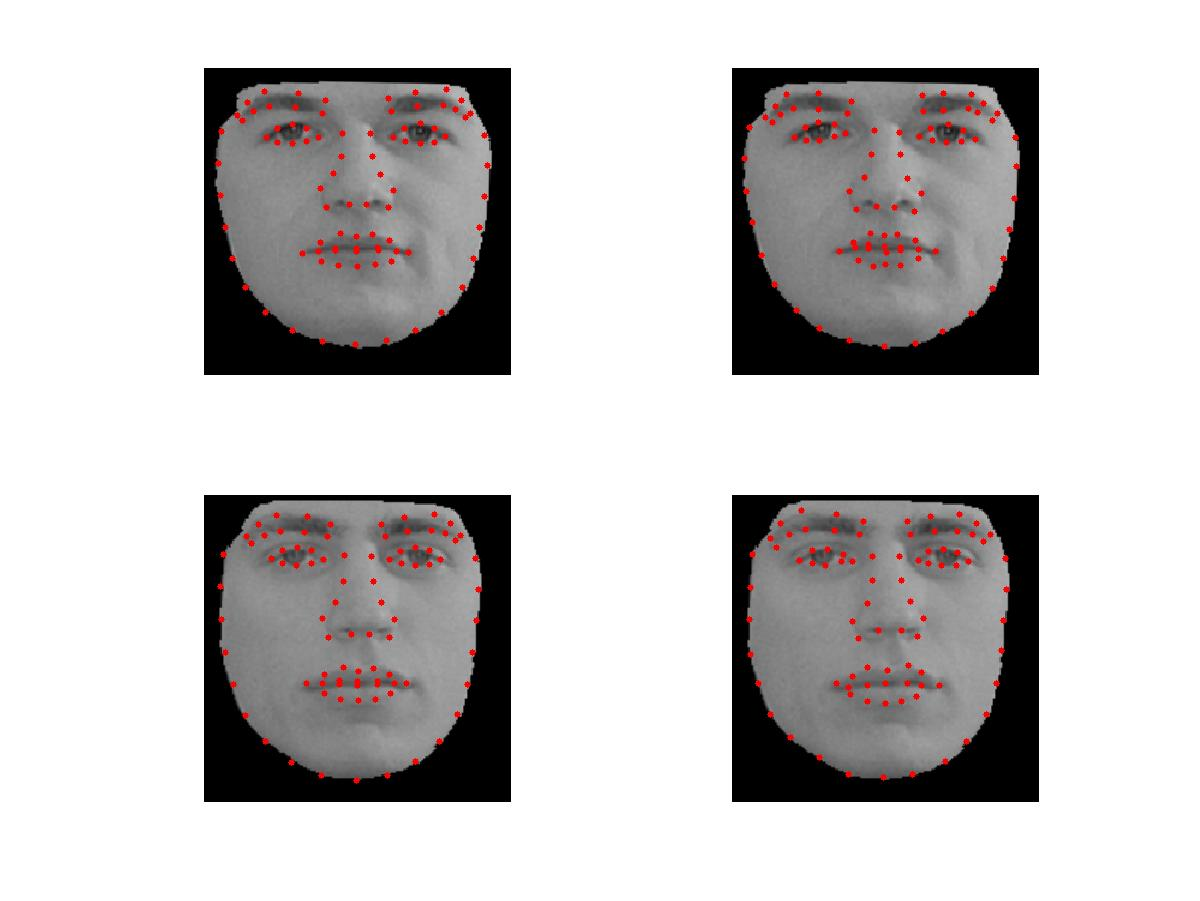
\includegraphics[scale=0.18]{b_com_face_lm1.jpg}
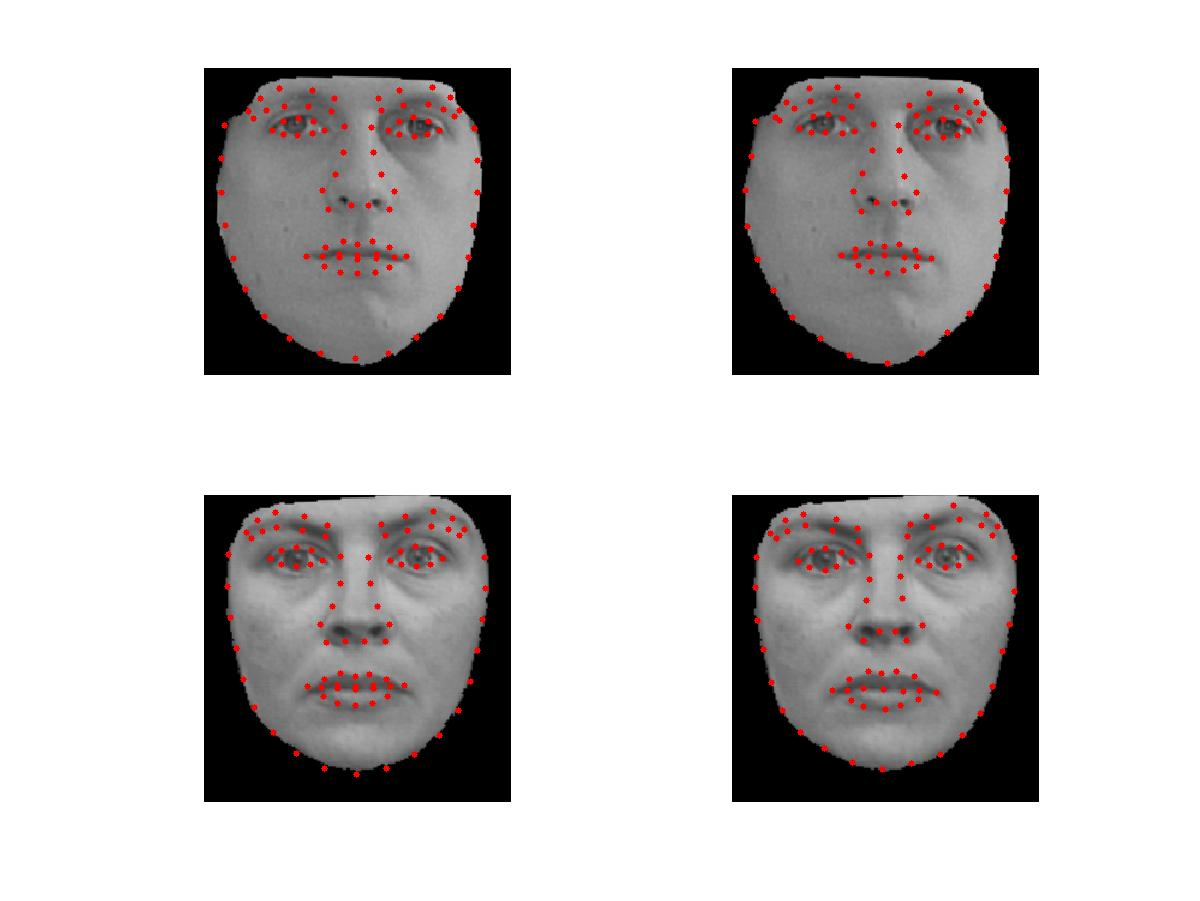
\includegraphics[scale=0.18]{b_com_face_lm2.jpg}
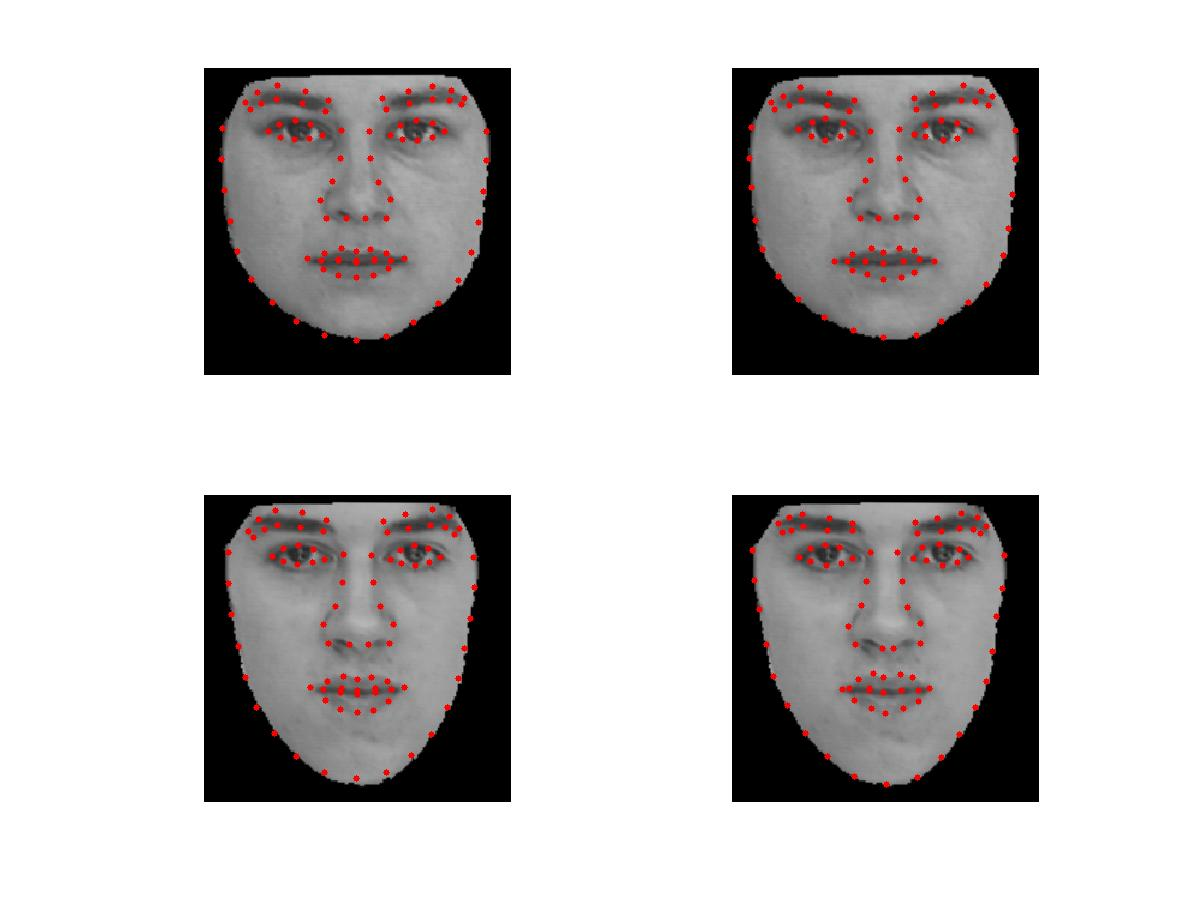
\includegraphics[scale=0.18]{b_com_face_lm3.jpg}
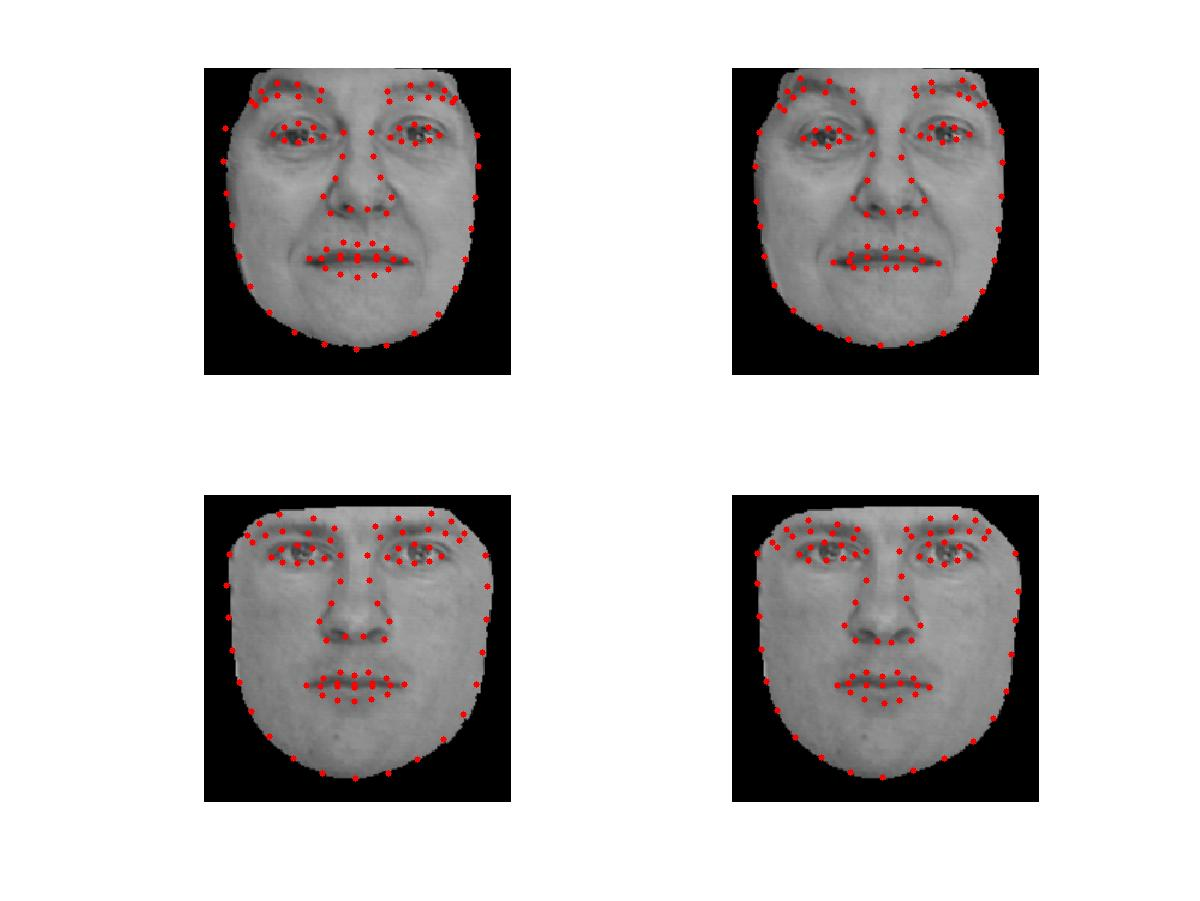
\includegraphics[scale=0.18]{b_com_face_lm4.jpg}
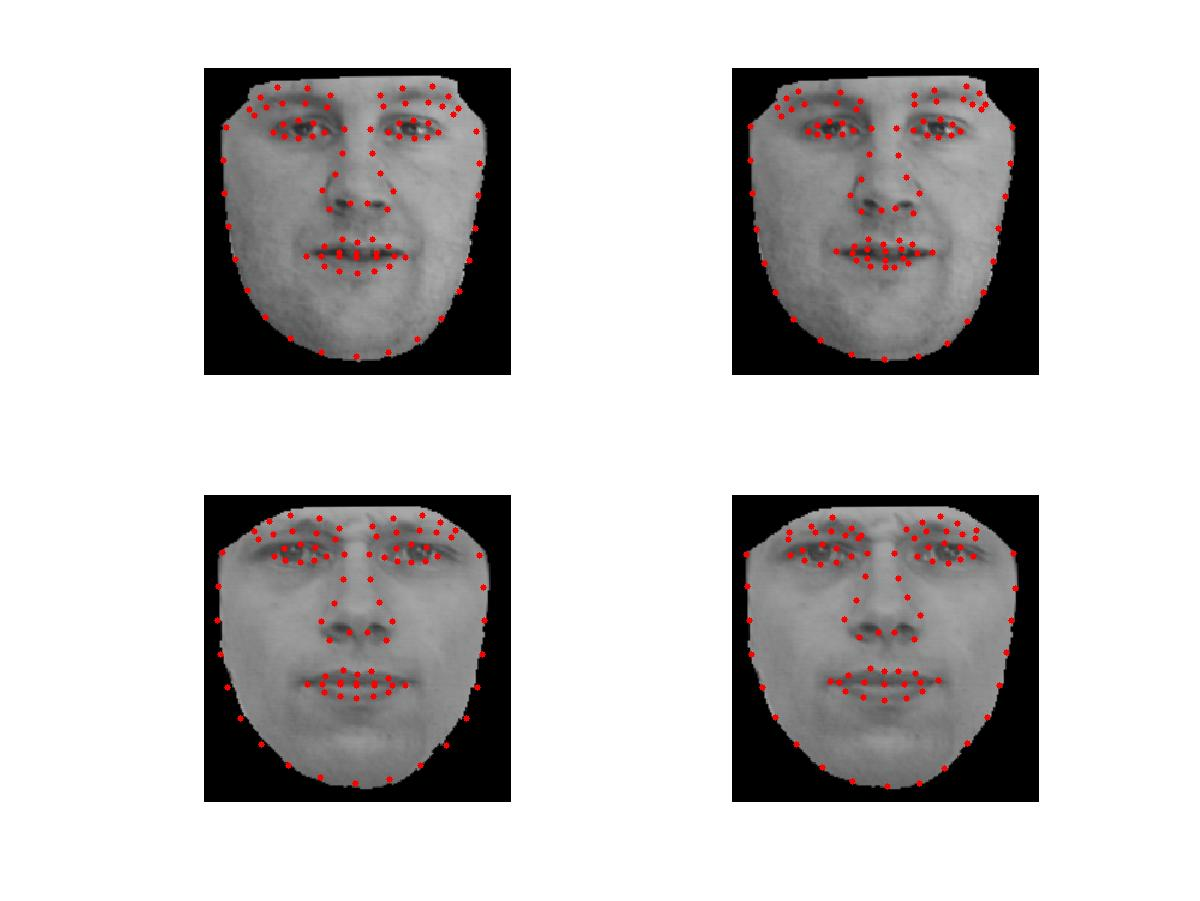
\includegraphics[scale=0.18]{b_com_face_lm5.jpg}
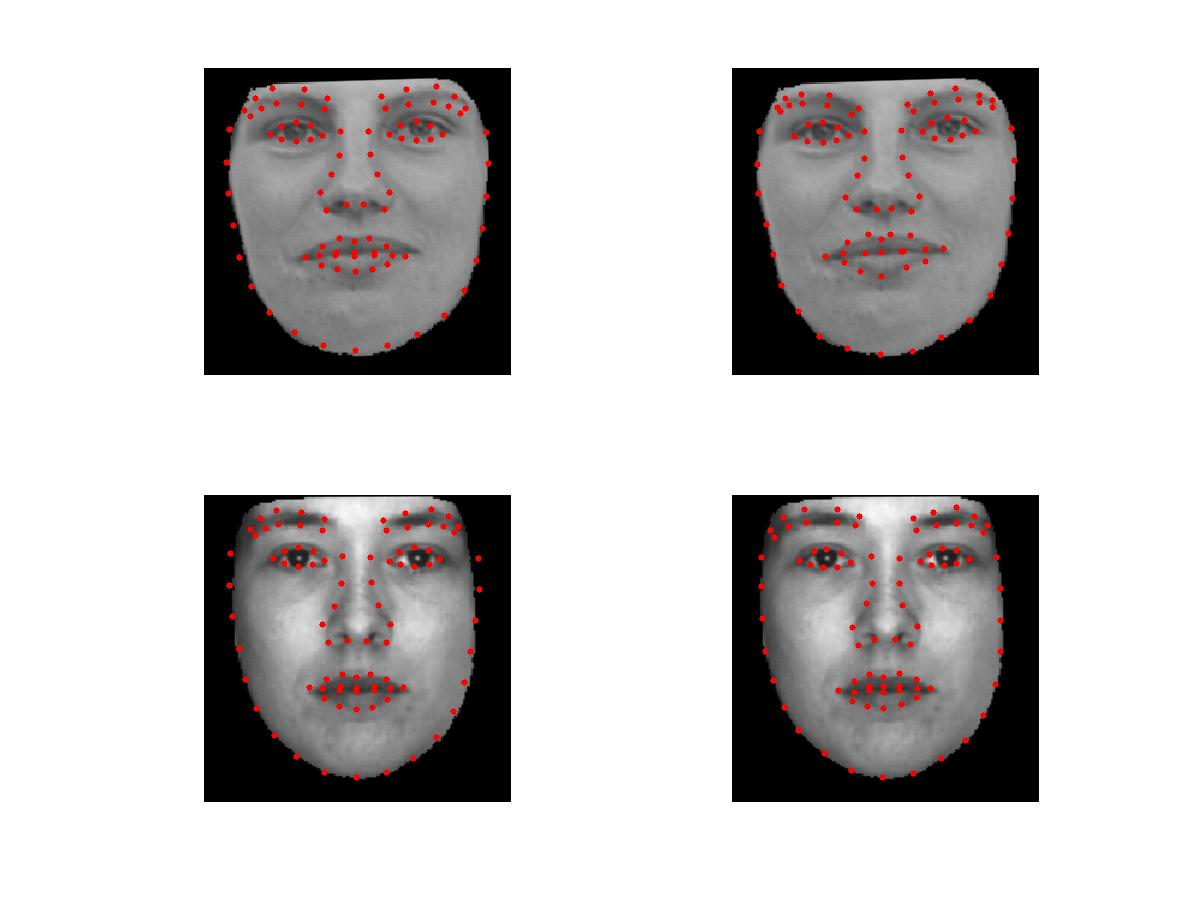
\includegraphics[scale=0.18]{b_com_face_lm6.jpg}
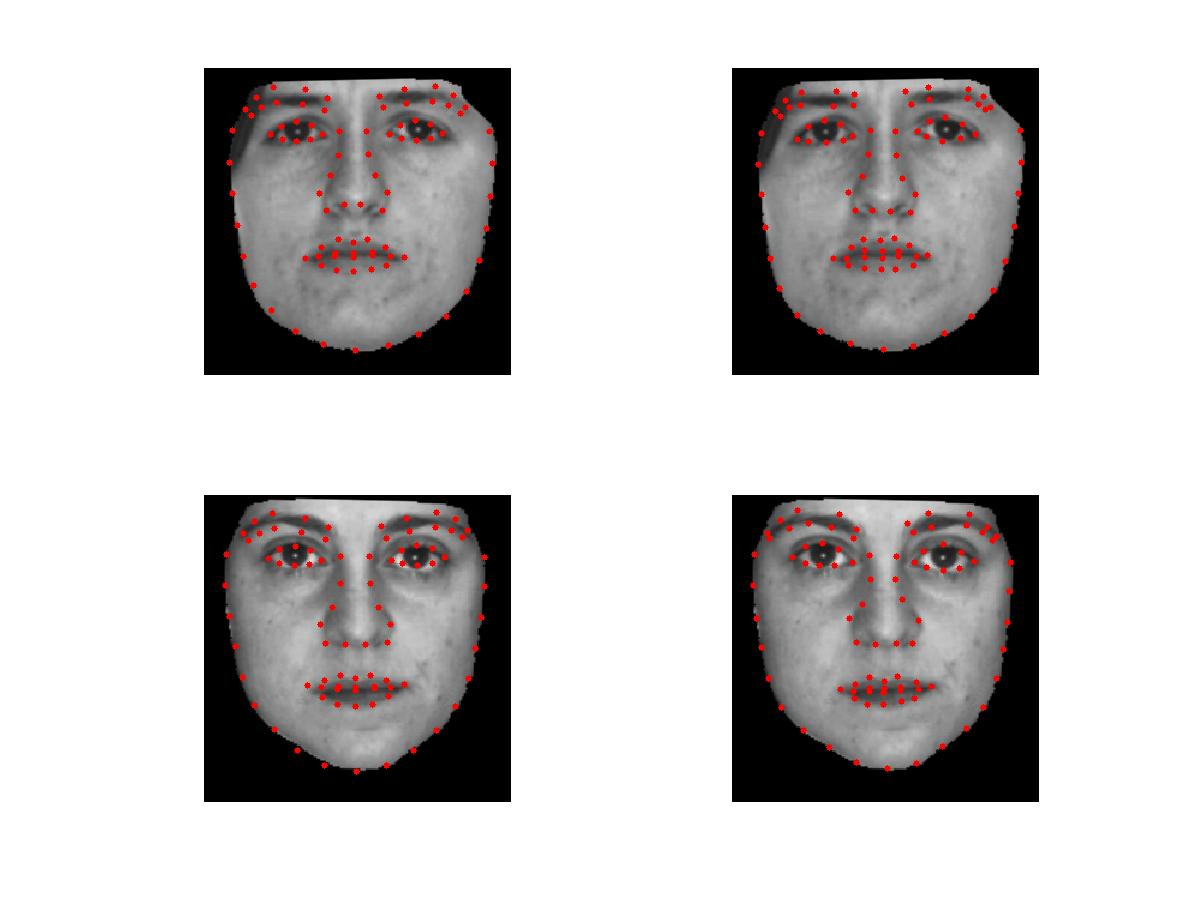
\includegraphics[scale=0.18]{b_com_face_lm7.jpg}
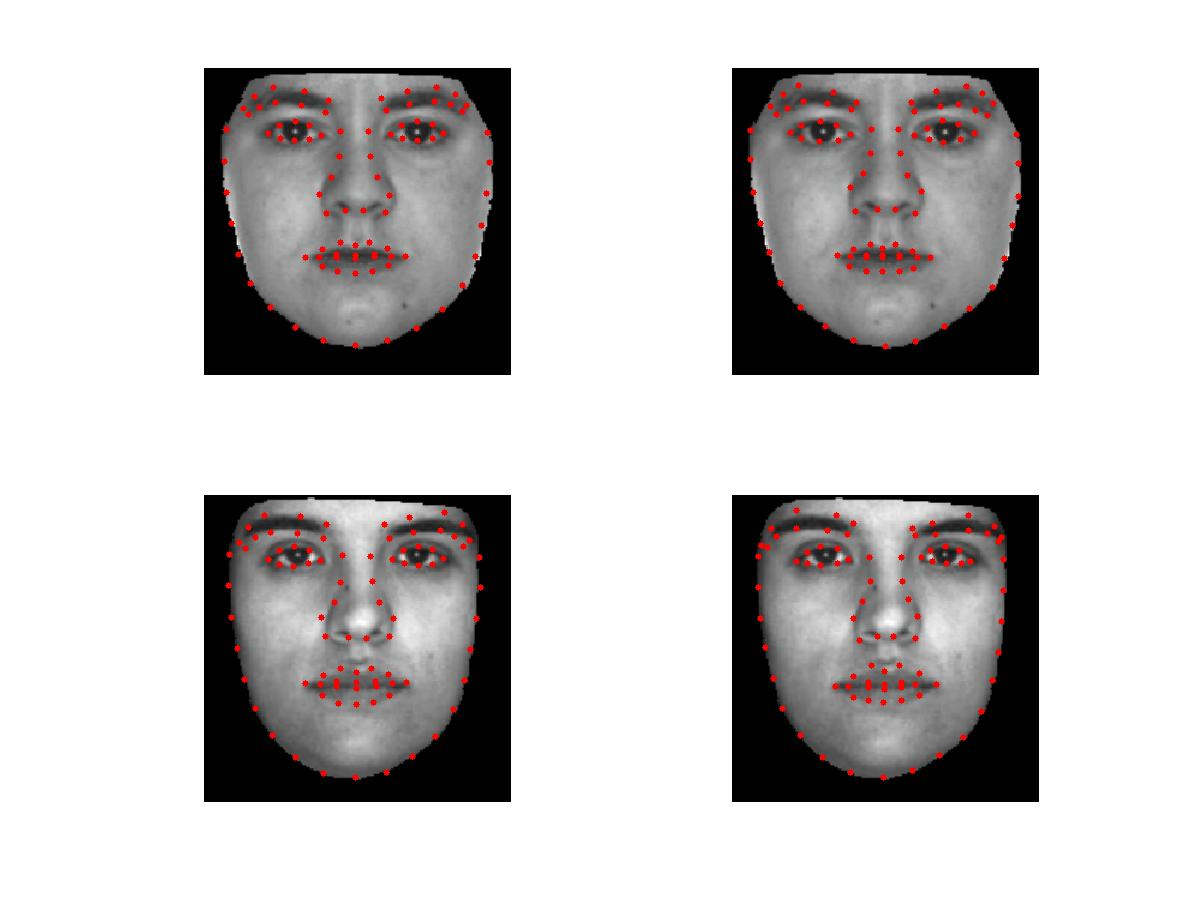
\includegraphics[scale=0.18]{b_com_face_lm8.jpg}
  \caption{mean face with mean landmark}
\end{figure}

\begin{figure}[H]
  \centering
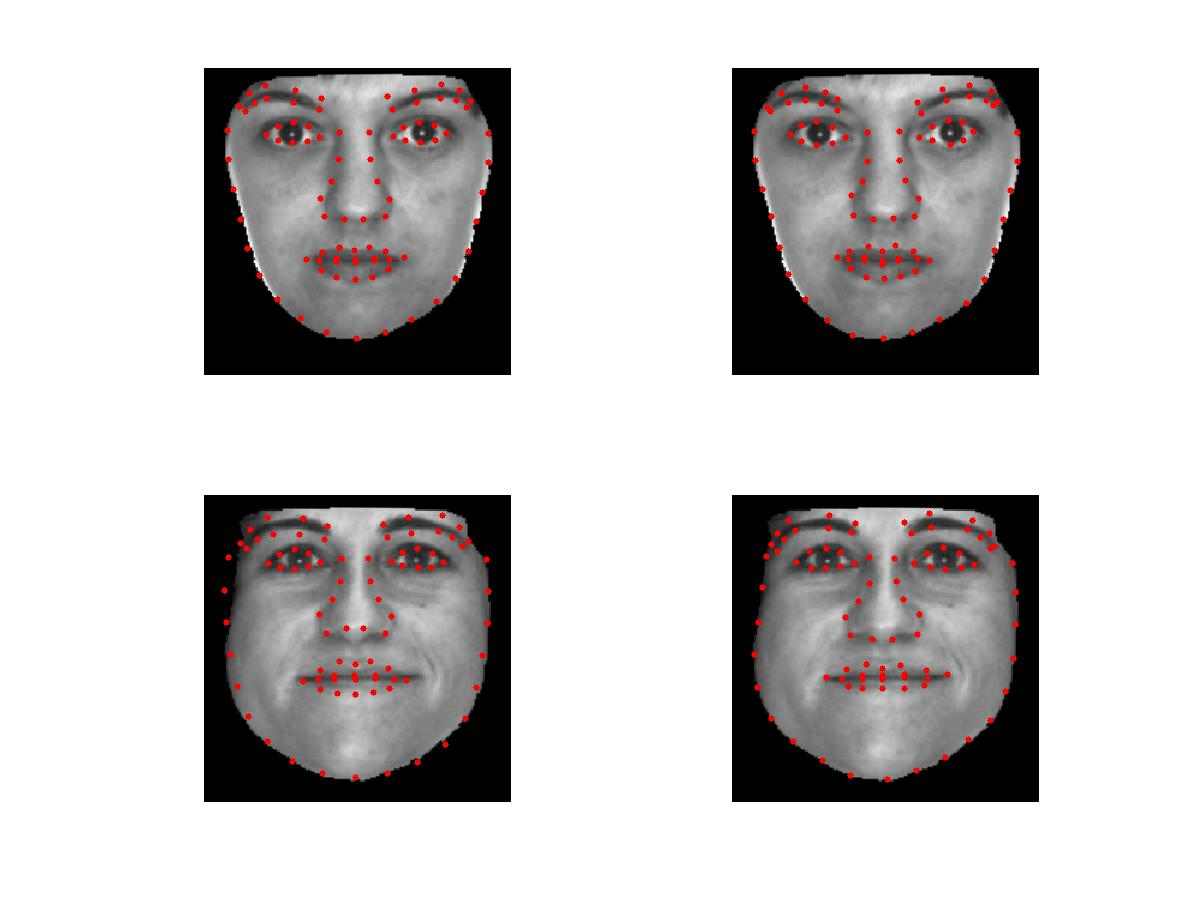
\includegraphics[scale=0.18]{b_com_face_lm9.jpg}
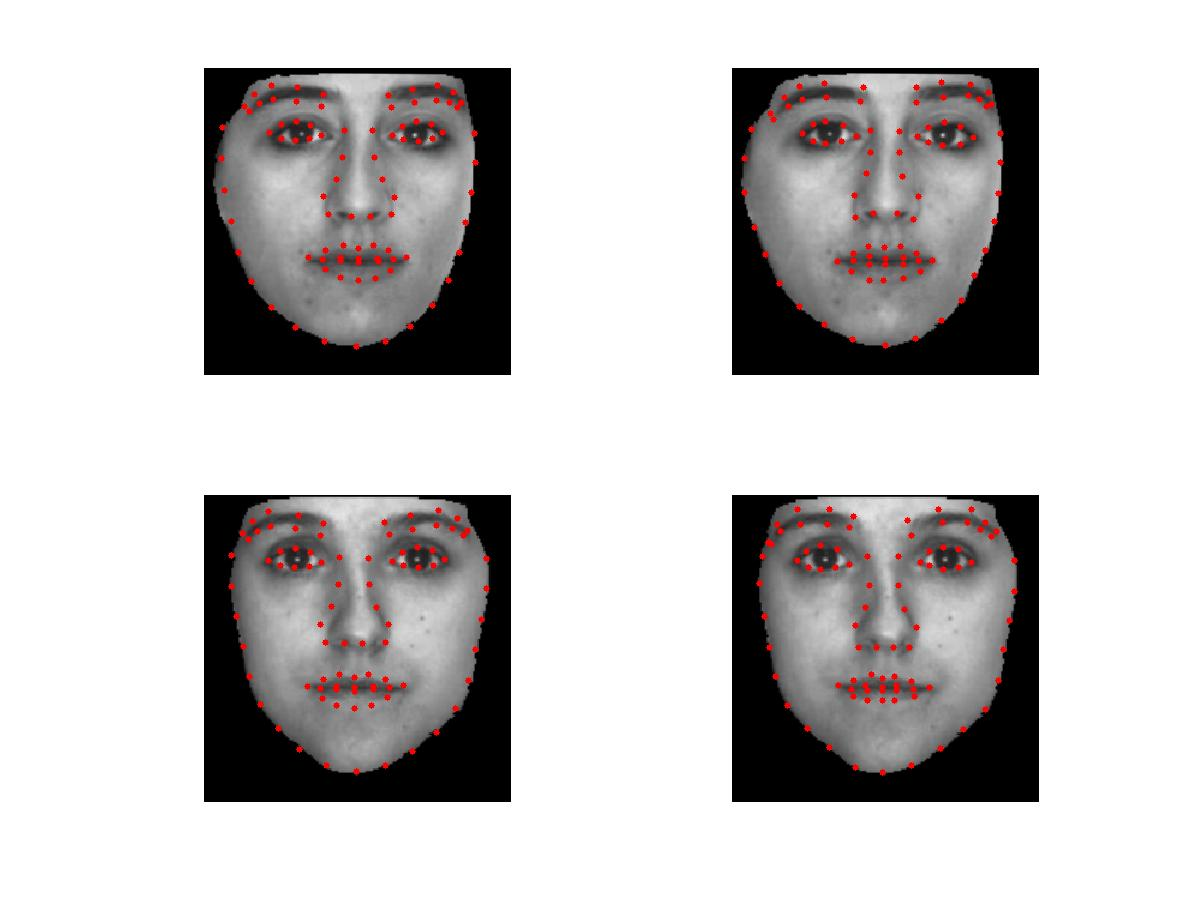
\includegraphics[scale=0.18]{b_com_face_lm10.jpg}
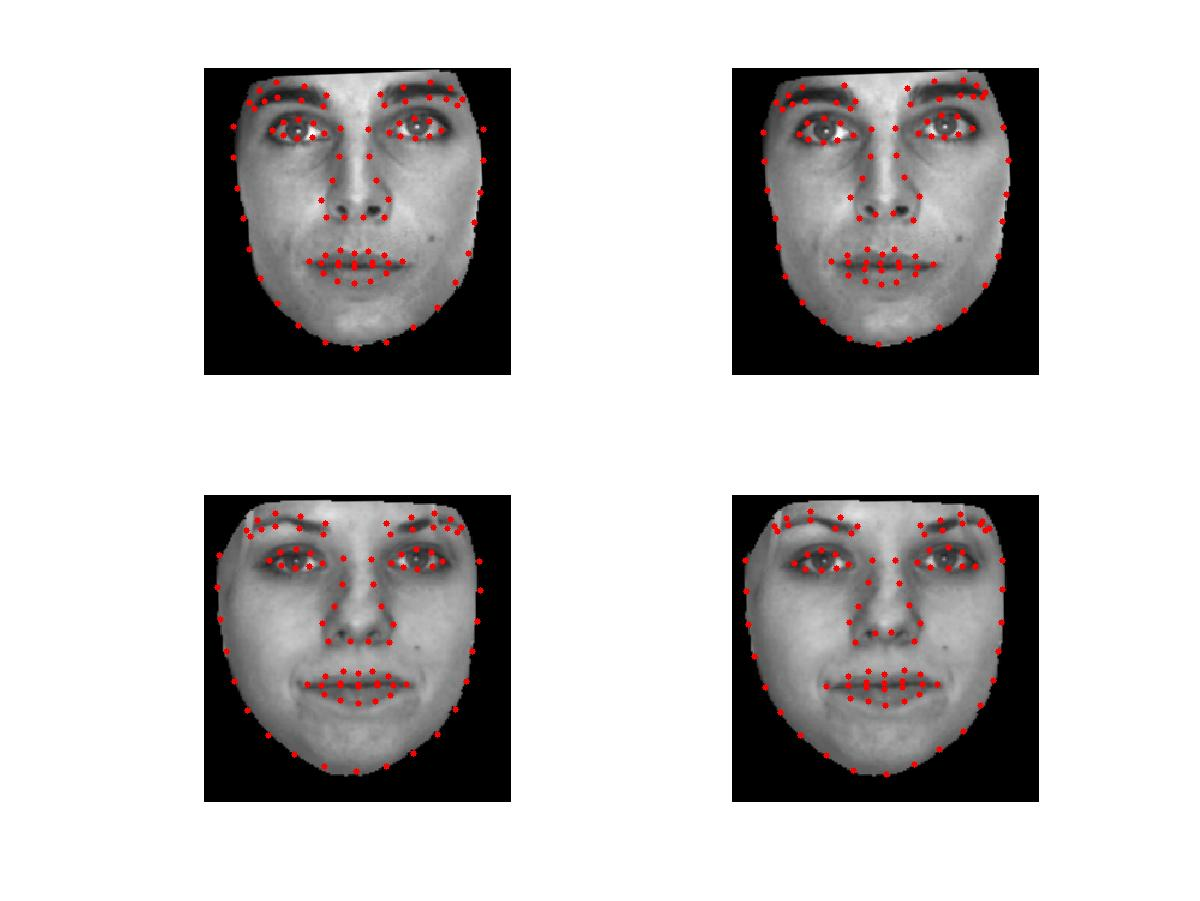
\includegraphics[scale=0.18]{b_com_face_lm11.jpg}
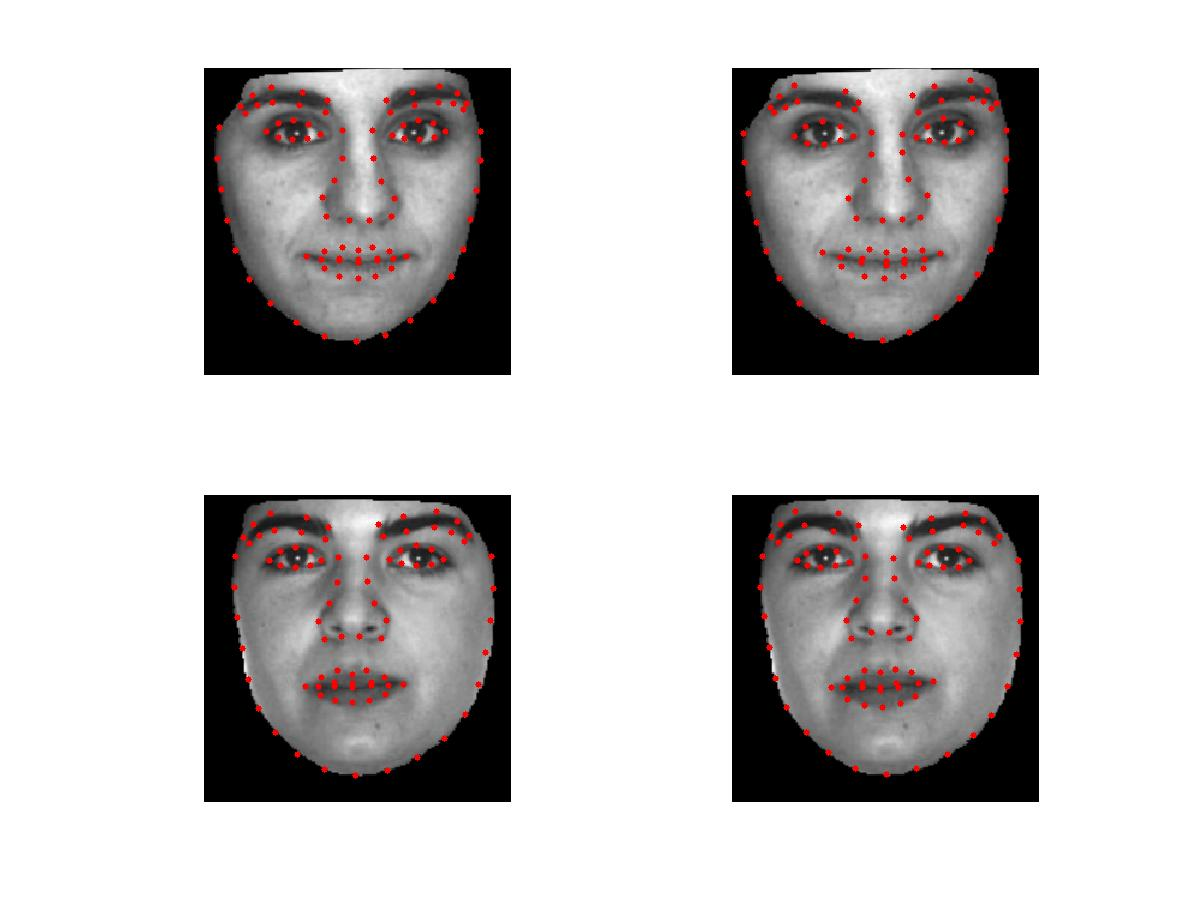
\includegraphics[scale=0.18]{b_com_face_lm12.jpg}
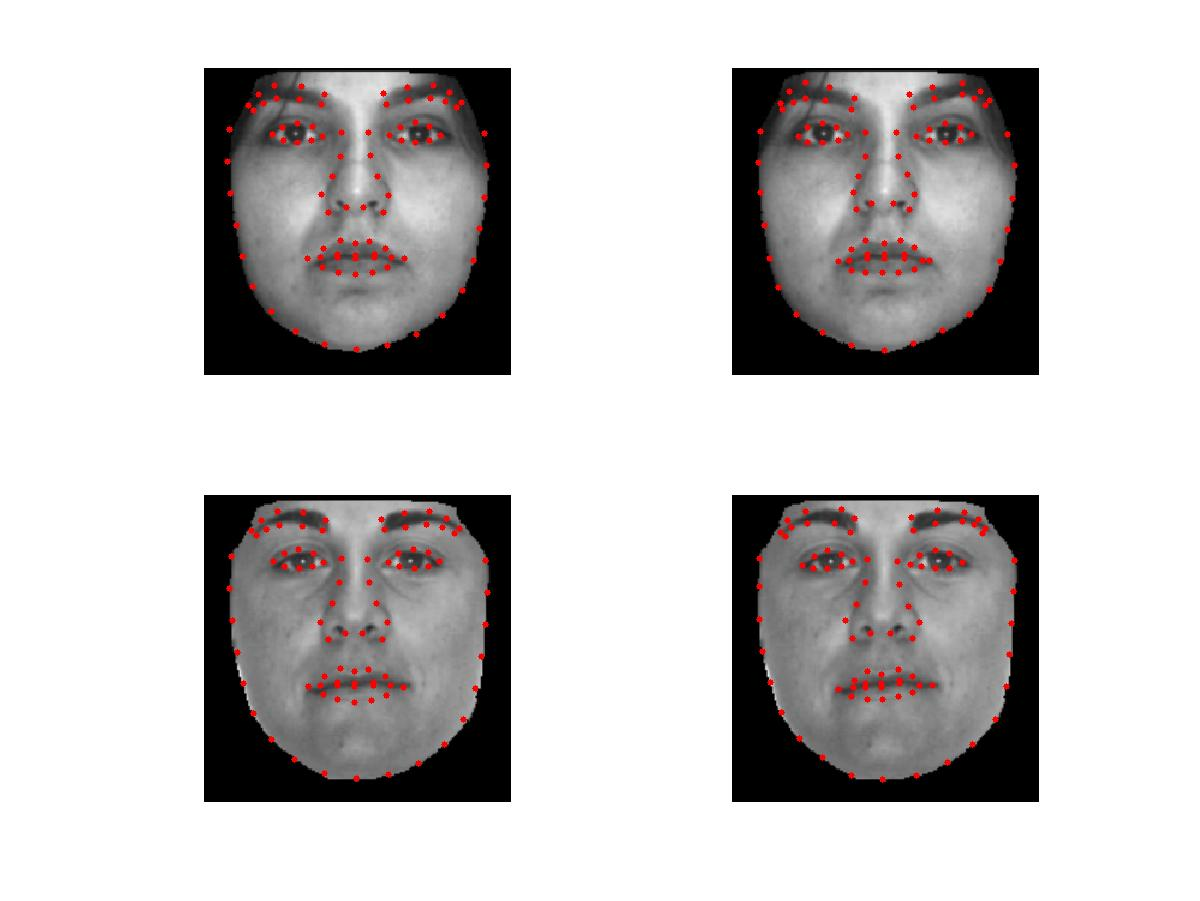
\includegraphics[scale=0.18]{b_com_face_lm13.jpg}
  \caption{mean face with mean landmark}
\end{figure}

The reconstruction error follows $e = \frac{1}{|Data|} \sum_{x \in Data} ||x - x_{rec}|| / D$. Figure.9 shows the results. 
\begin{figure}[H]
  \centering
  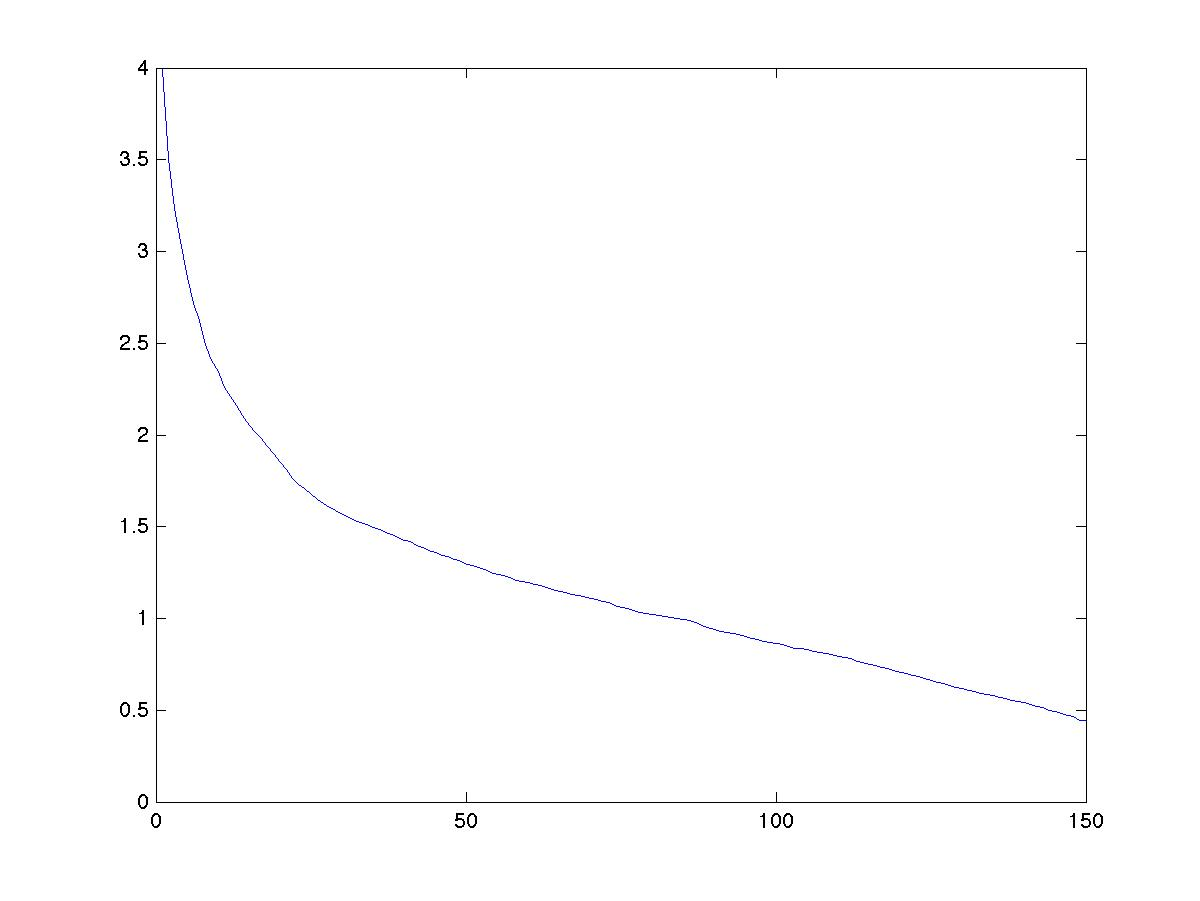
\includegraphics[scale=0.2]{b_reconstructerror_lm.jpg}
  \caption{Reconstruct Error for landmark}
\end{figure}

\item
The idea is to combine the two steps above to improve the precision of reconstruction face. First, we calculate the PCA of aligned images and PCA of landmark. We have been showed the PCA of landmarks in (2). Figure.10 shows the first ten eigen aligned faces. 
\begin{figure}[H]
  \centering
  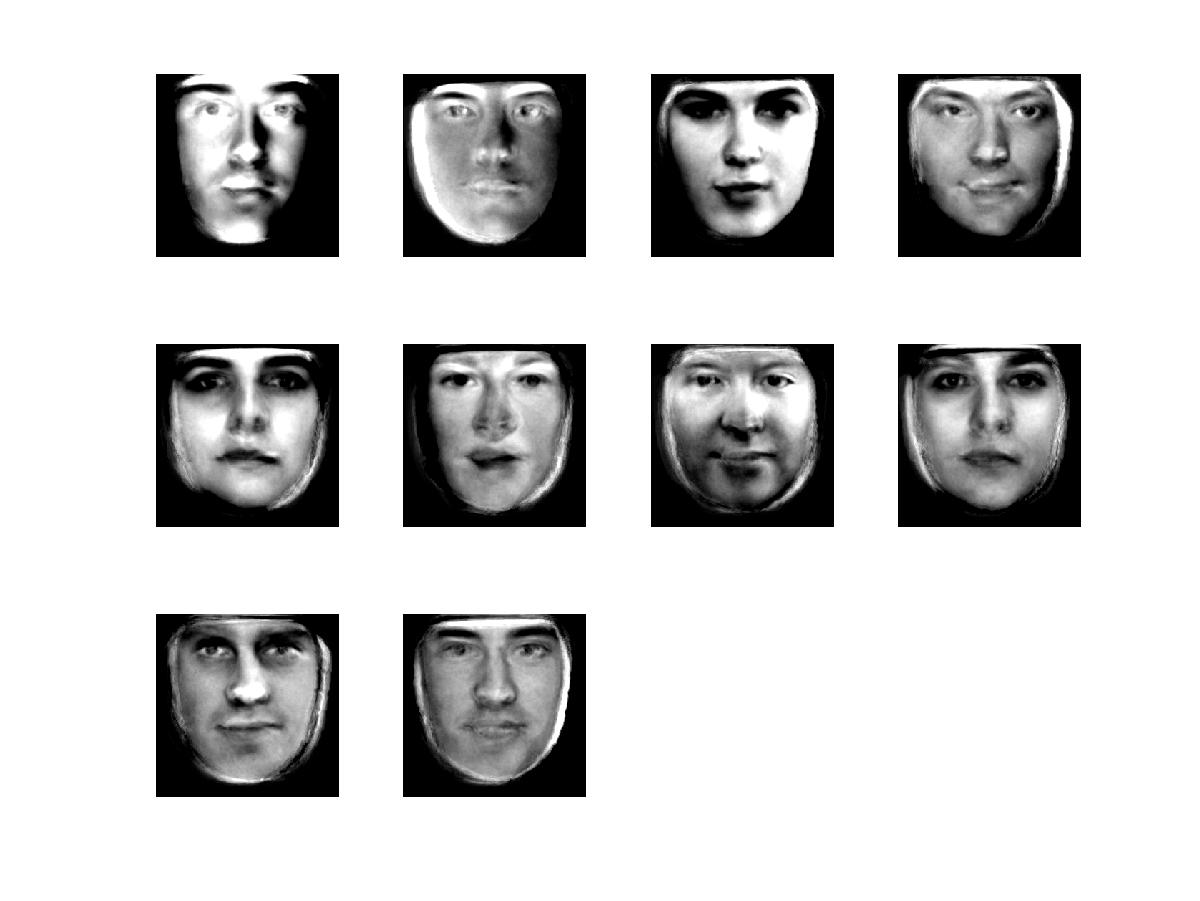
\includegraphics[scale=0.25]{c_eigenface_wf.jpg}
  \caption{Top 10 eigen aligned faces}
\end{figure}
Then for each test data $\{I, L\}$, where $I$ is original image of face, $L$ is original landmark. 1) project the $L$ to top 10 eigen-warpings, then we can get the reconstructed landmarks $L_{rec}$. 2) Warp the $\{I, L\}$ to the mean position $\mu_L$, $\{I', \mu_L\}$, and project $I'$ to top k eigen-faces, we get the reconstructed image $I'_{rec}$ for $I'$. 3) Warp the reconstructed faces $\{I'_{rec}, \mu_L\}$ to the position that reconstructed in 1), then we get $\{I_{rec}, L_{rec}\}$. 

Figure.11, 12 and Figure.13. show the comparisons between reconstructed faces and original faces. The left side of each pari faces is reconstructed faces and the right side is original face. 
\begin{figure}[H]
  \centering
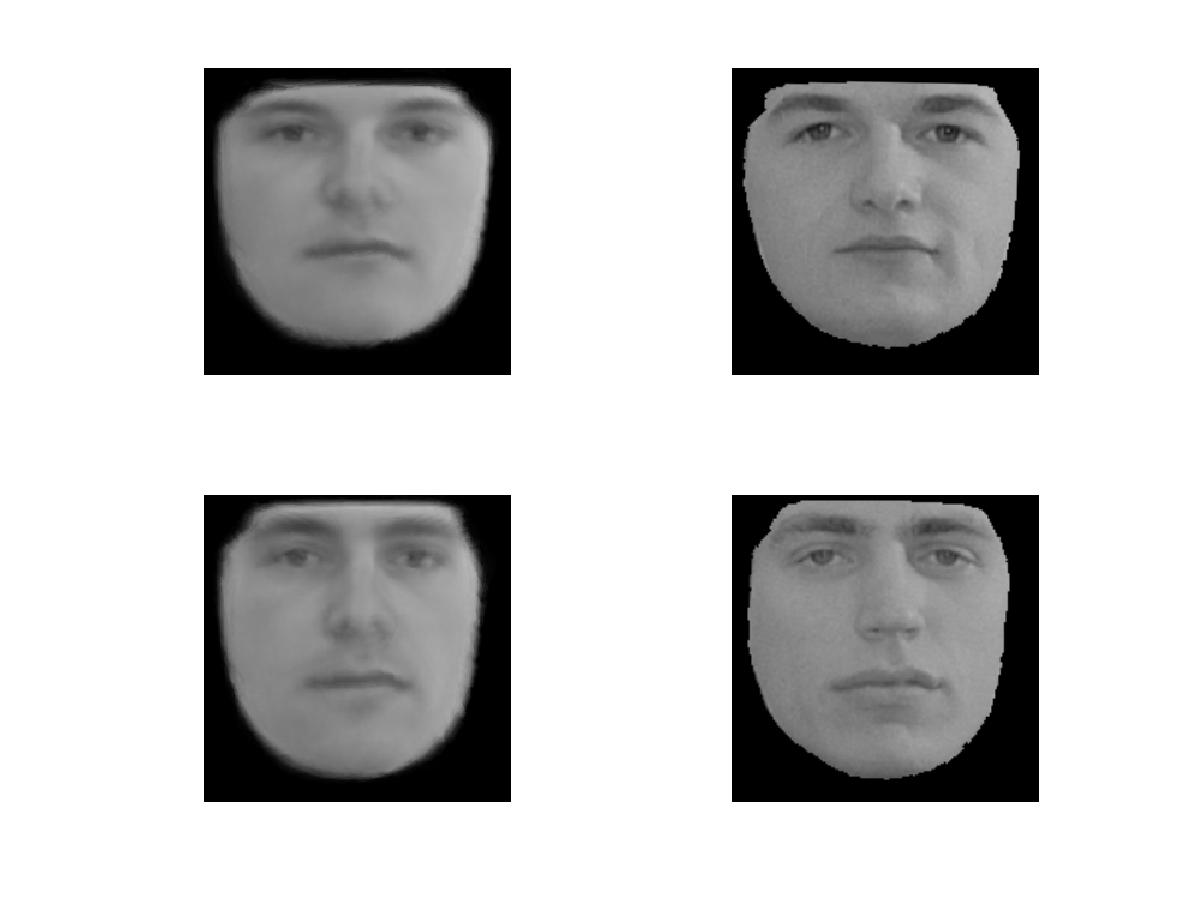
\includegraphics[scale=0.18]{c_rec_face_wf1.jpg}
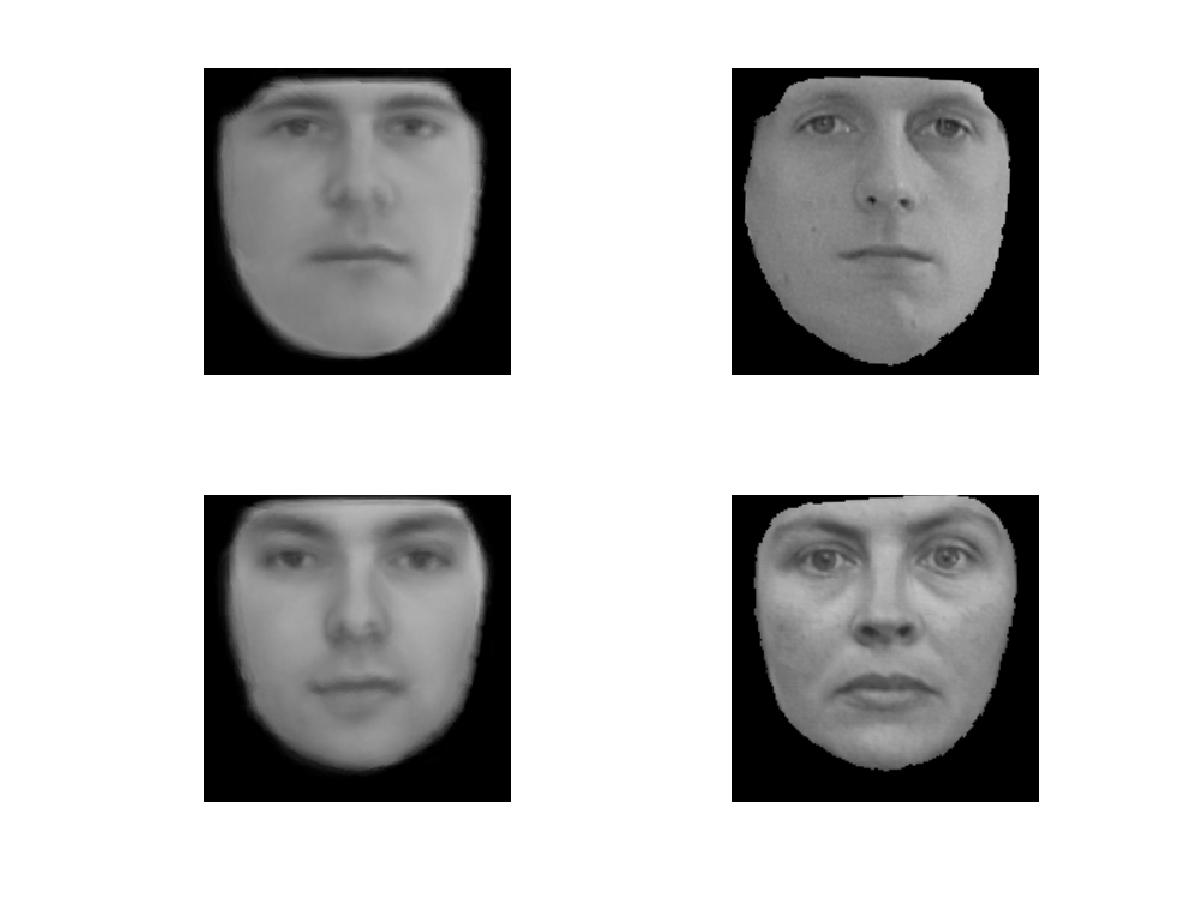
\includegraphics[scale=0.18]{c_rec_face_wf2.jpg}
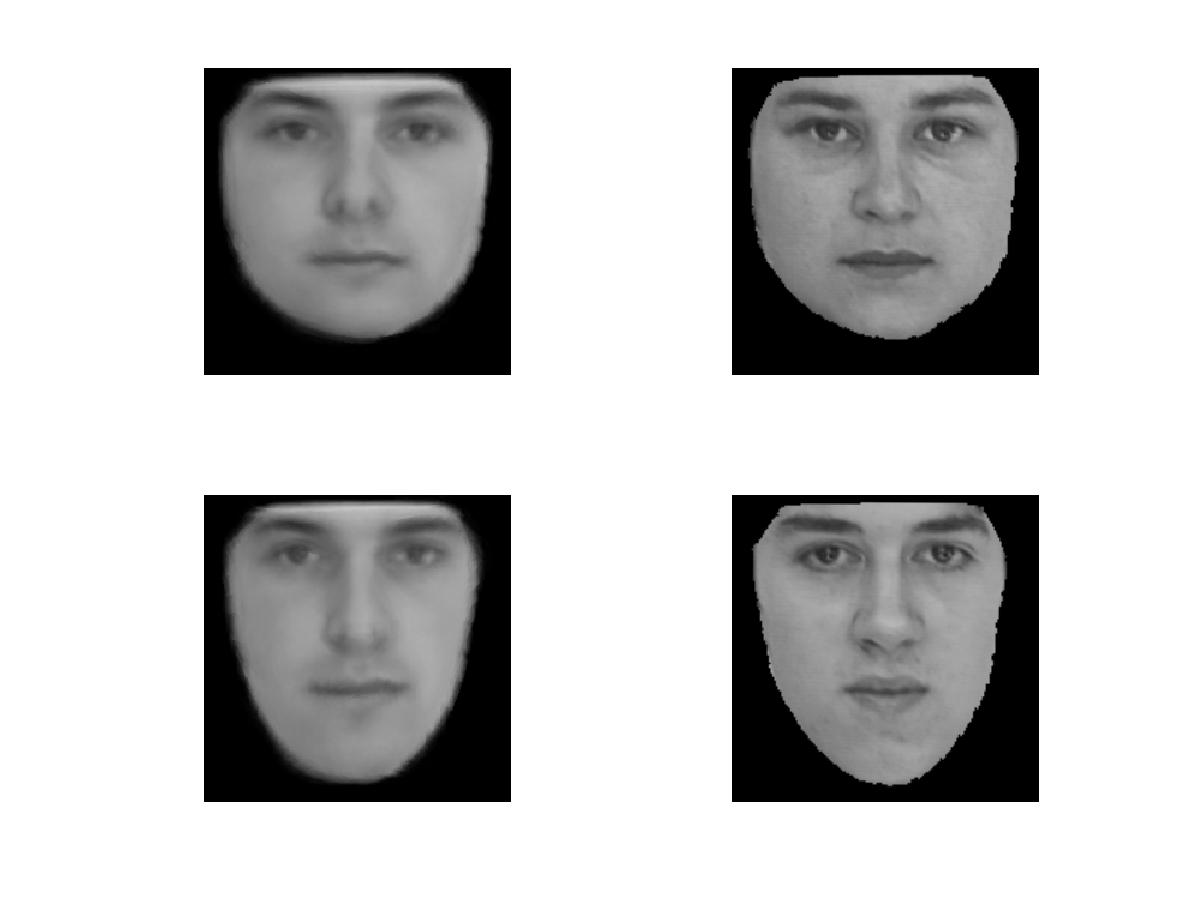
\includegraphics[scale=0.18]{c_rec_face_wf3.jpg}
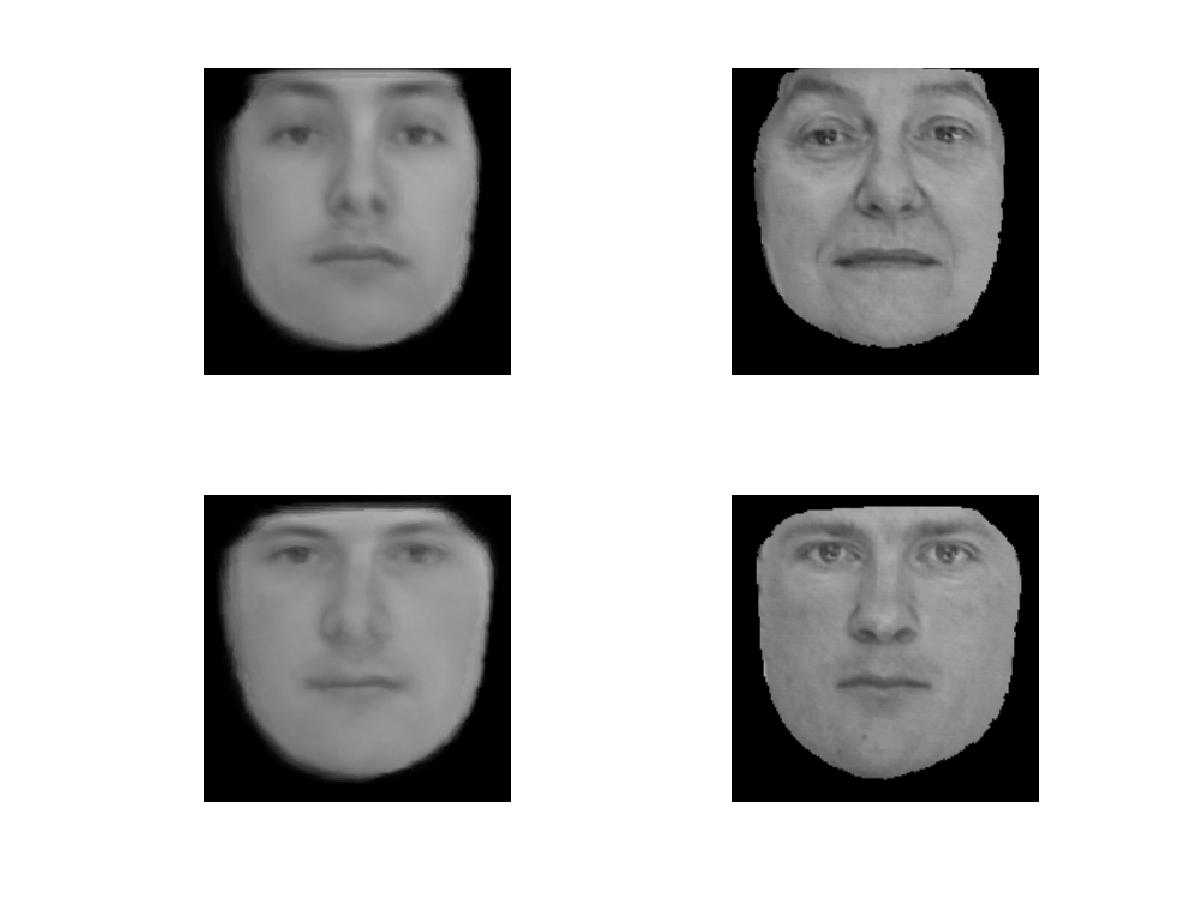
\includegraphics[scale=0.18]{c_rec_face_wf4.jpg}
  \caption{Reconstructed Faces}
\end{figure}

\begin{figure}[H]
  \centering
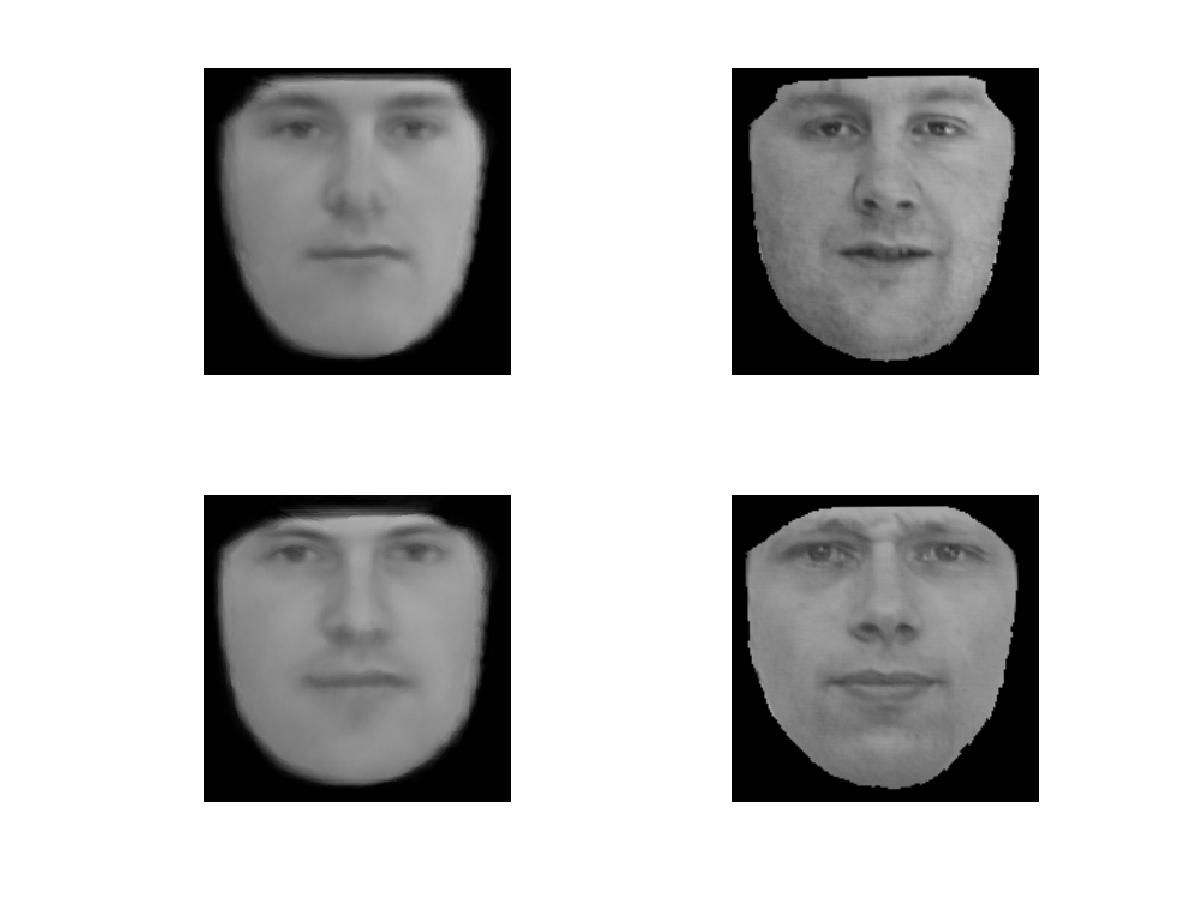
\includegraphics[scale=0.18]{c_rec_face_wf5.jpg}
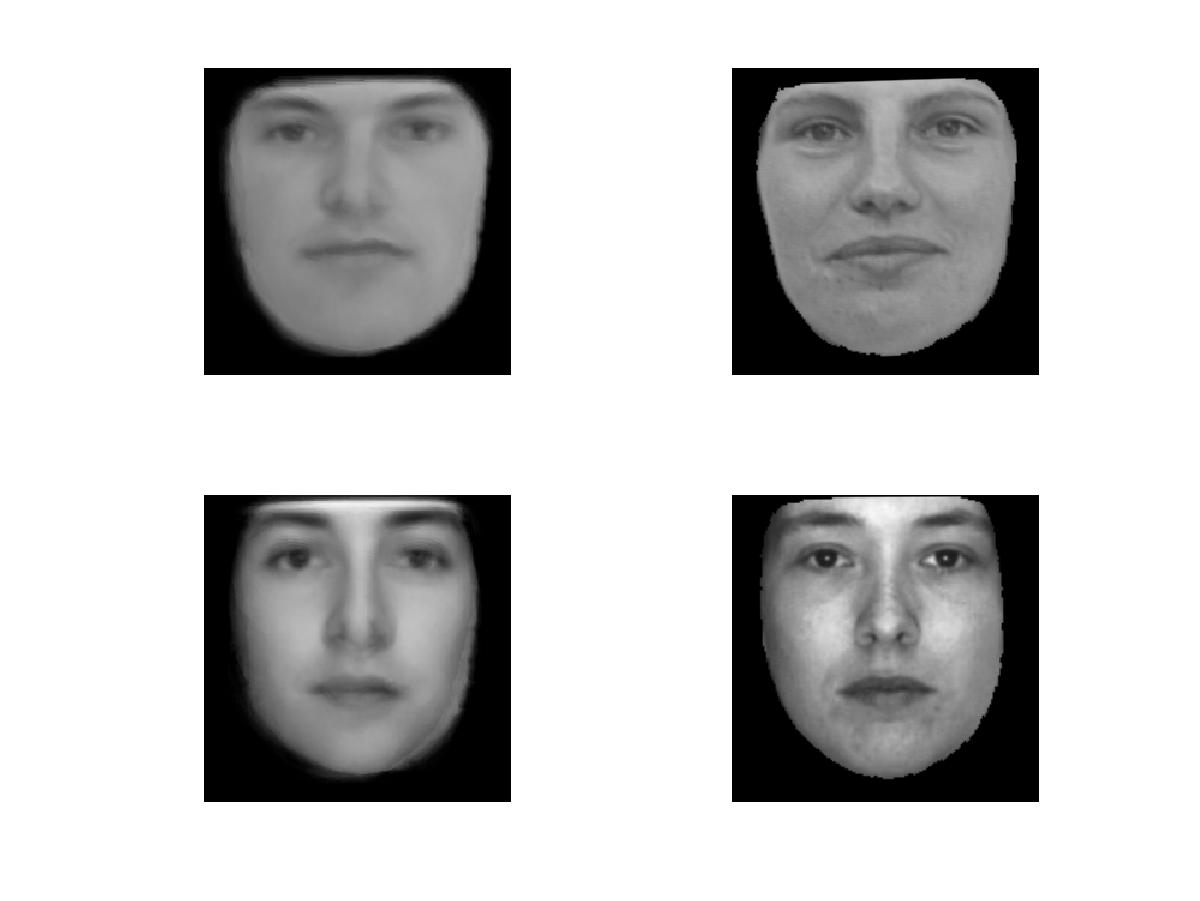
\includegraphics[scale=0.18]{c_rec_face_wf6.jpg}
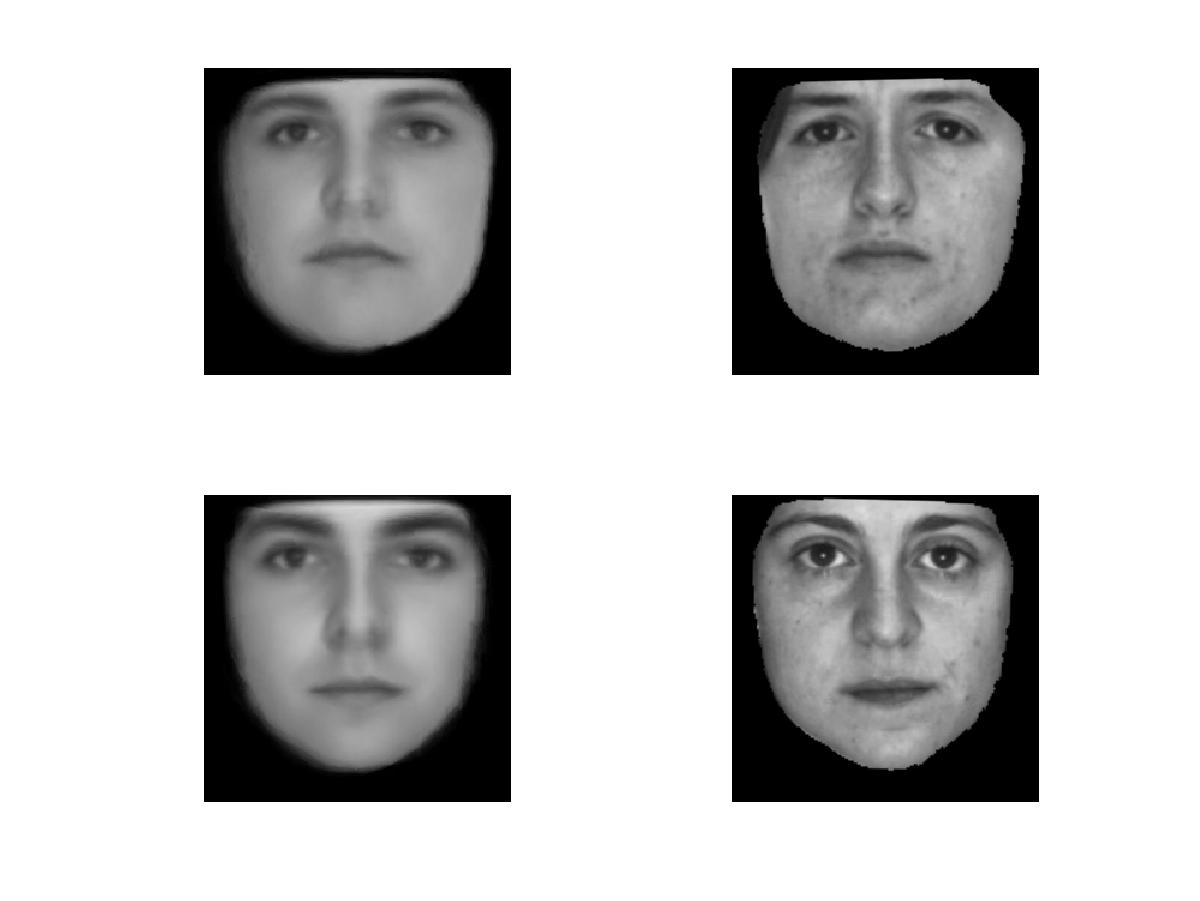
\includegraphics[scale=0.18]{c_rec_face_wf7.jpg}
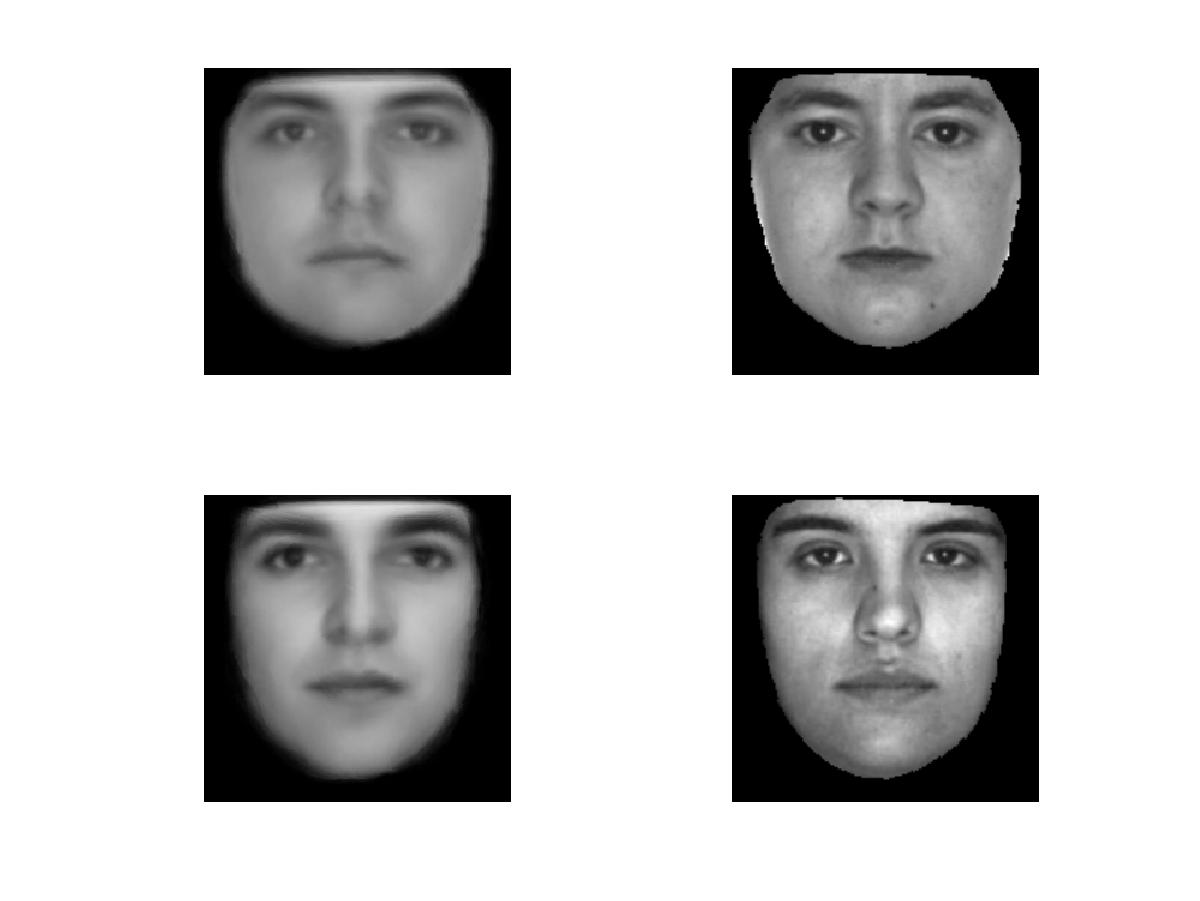
\includegraphics[scale=0.18]{c_rec_face_wf8.jpg}
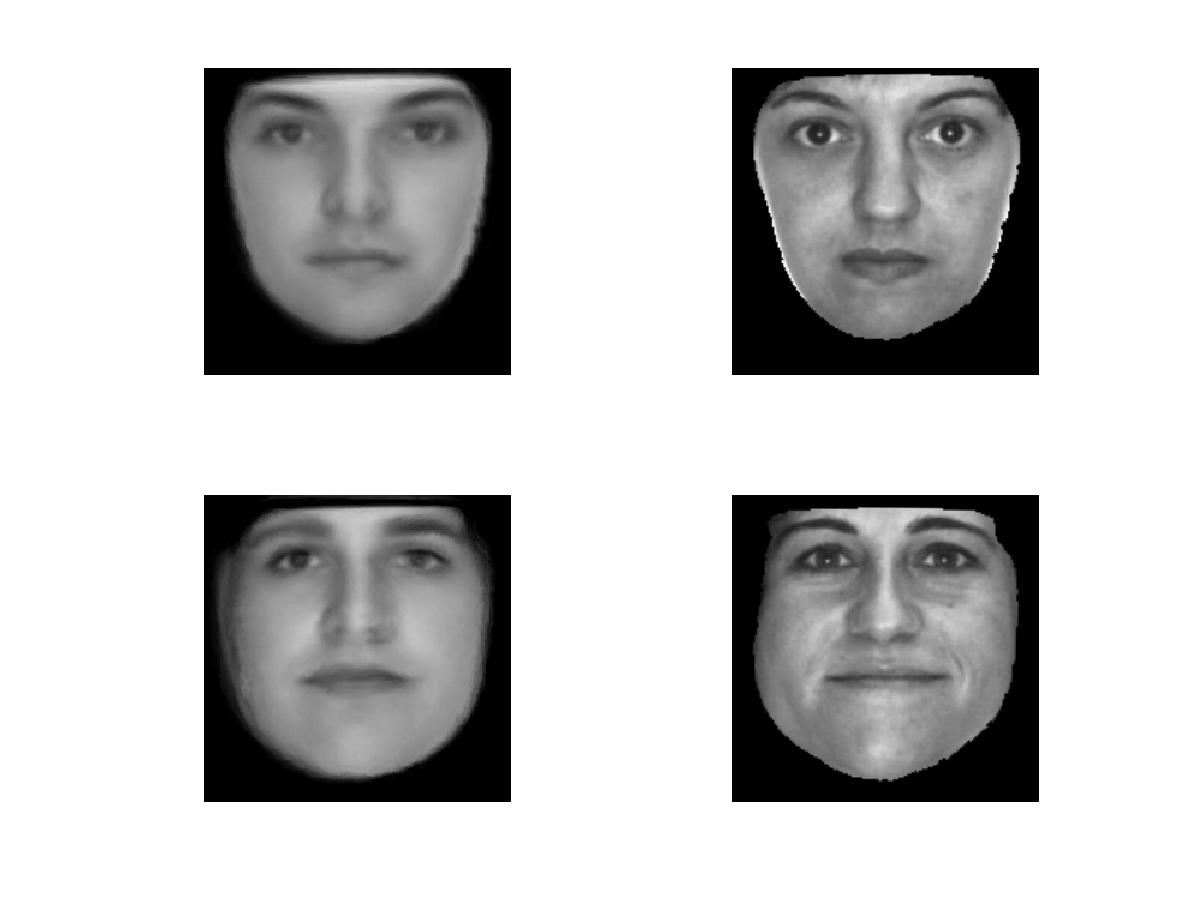
\includegraphics[scale=0.18]{c_rec_face_wf9.jpg}
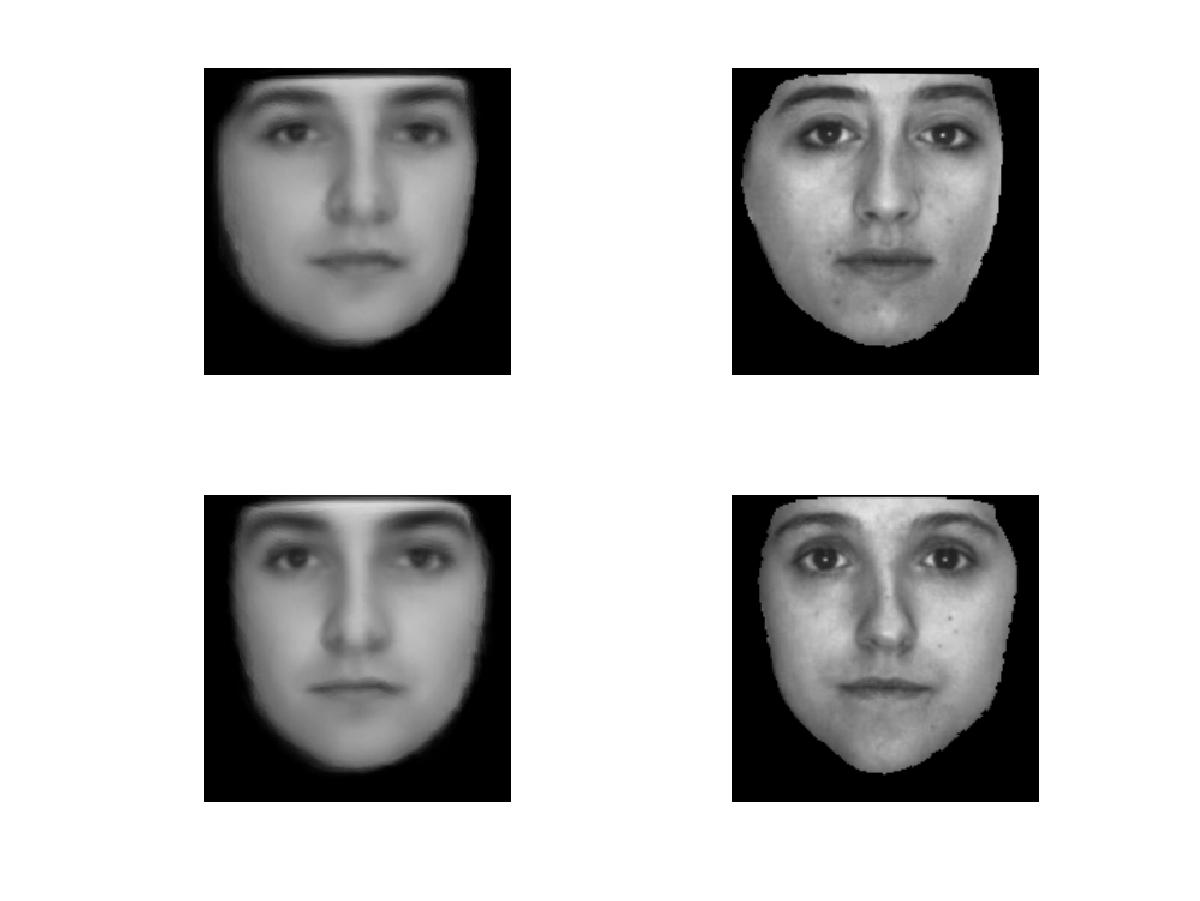
\includegraphics[scale=0.18]{c_rec_face_wf10.jpg}
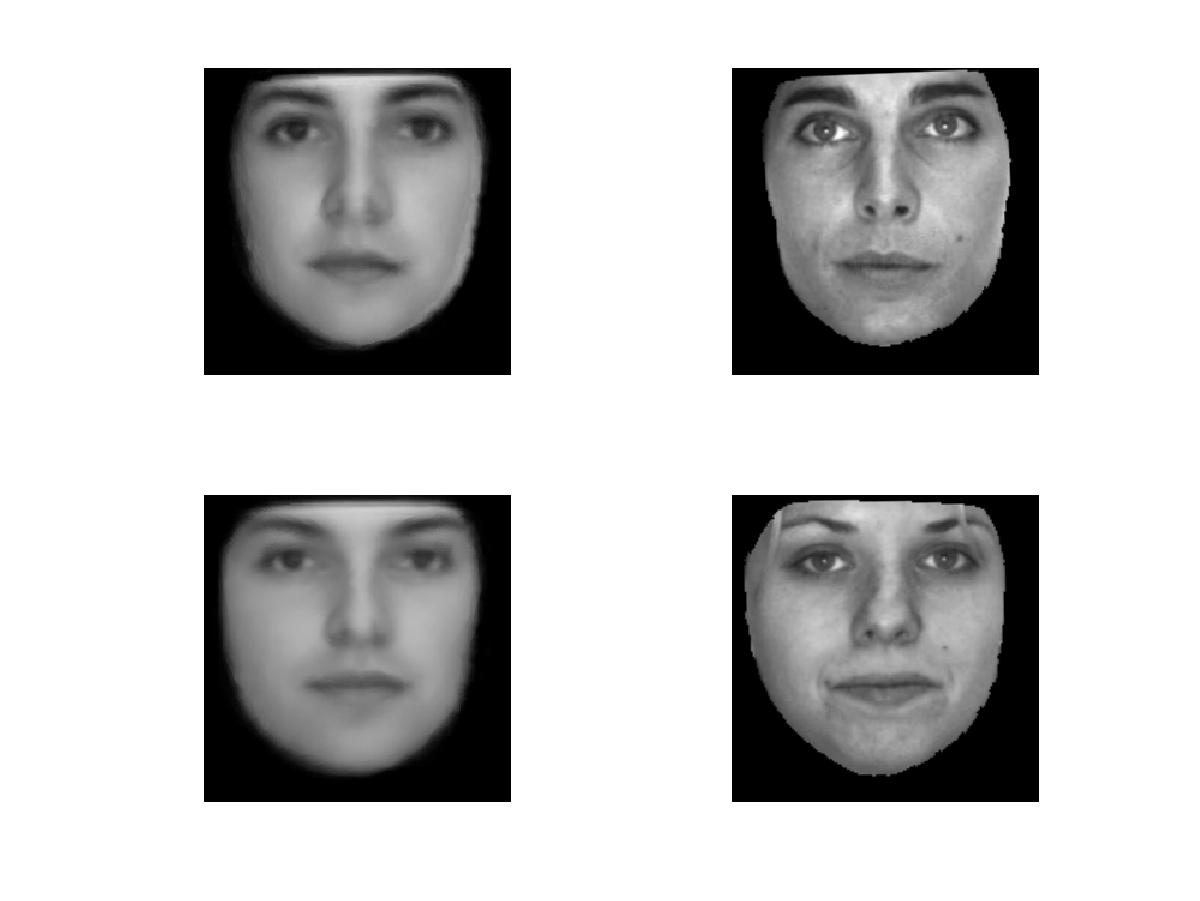
\includegraphics[scale=0.18]{c_rec_face_wf11.jpg}
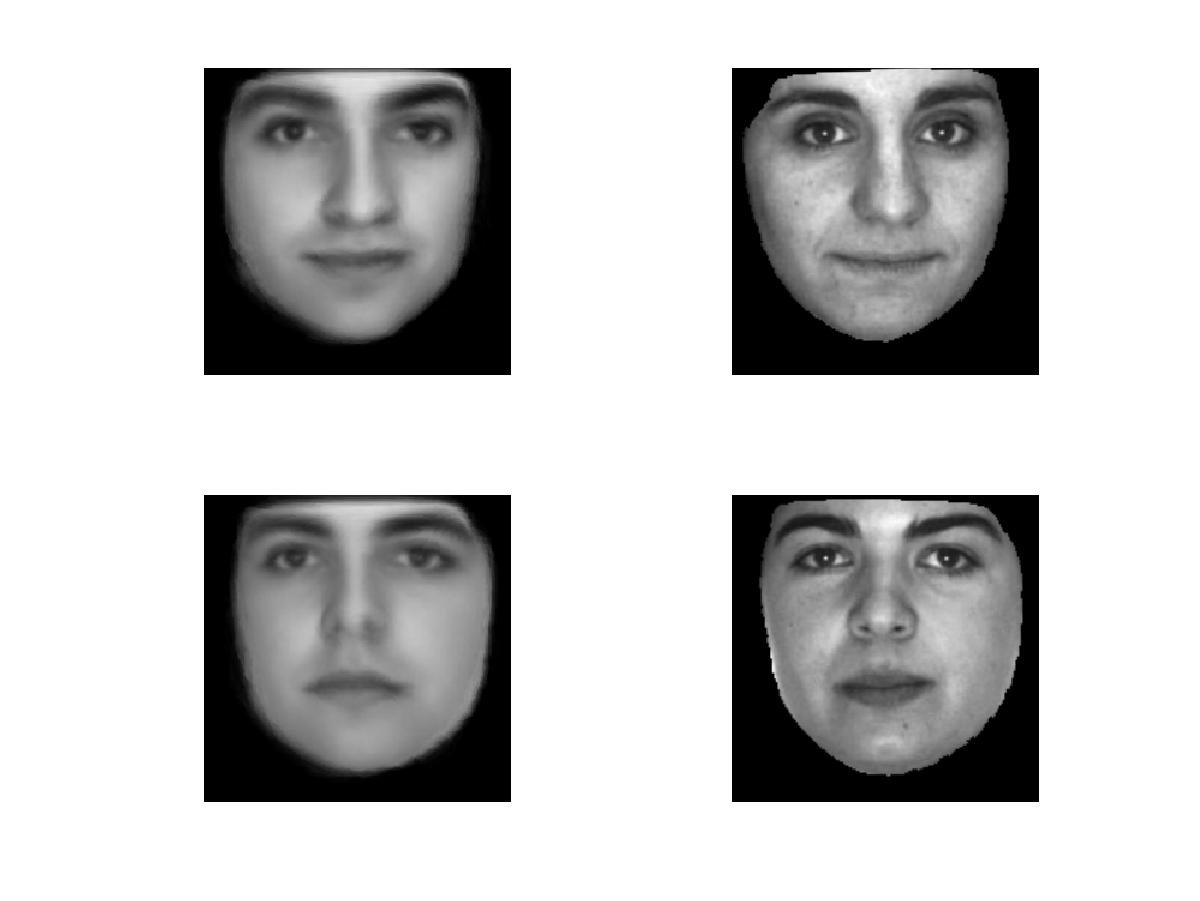
\includegraphics[scale=0.18]{c_rec_face_wf12.jpg}
  \caption{Reconstructed Faces}
\end{figure}

\begin{figure}[H]
  \centering
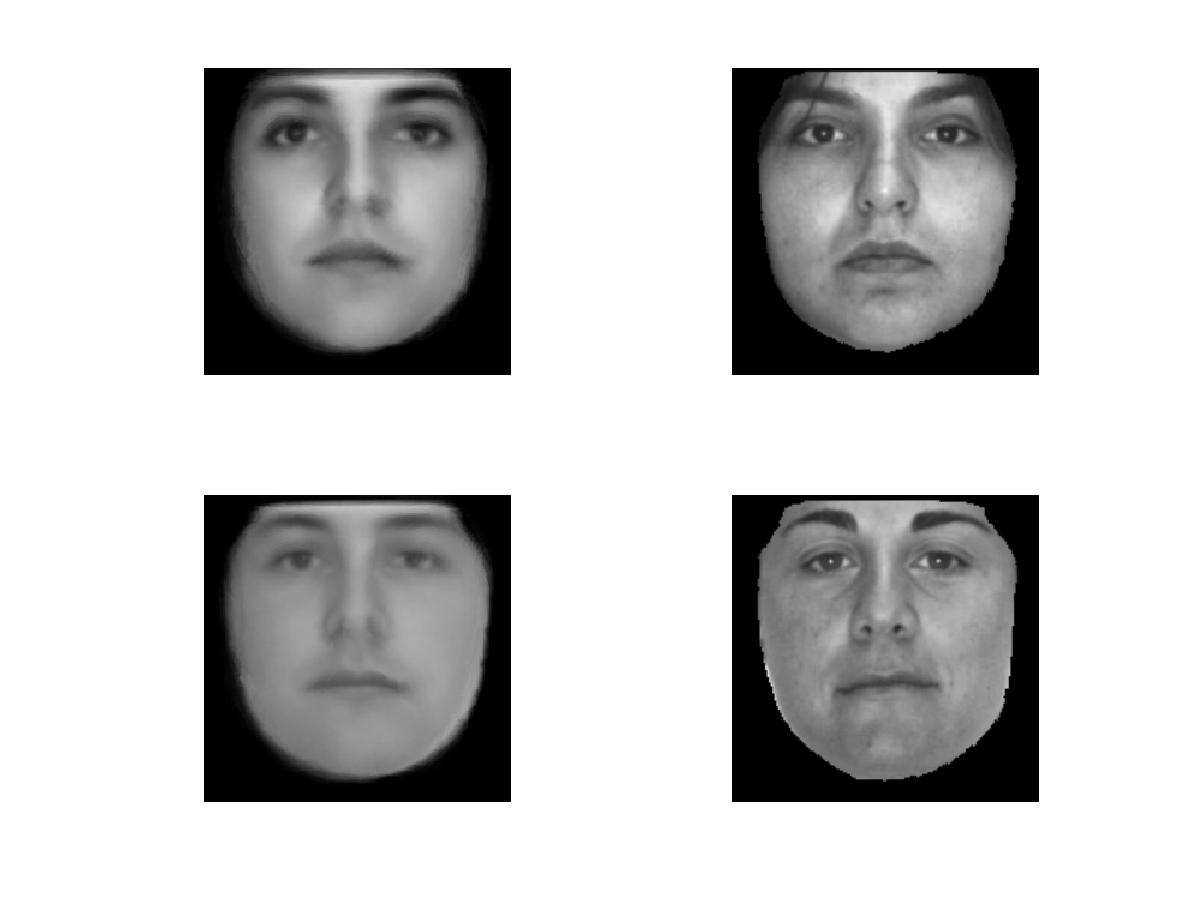
\includegraphics[scale=0.18]{c_rec_face_wf13.jpg}
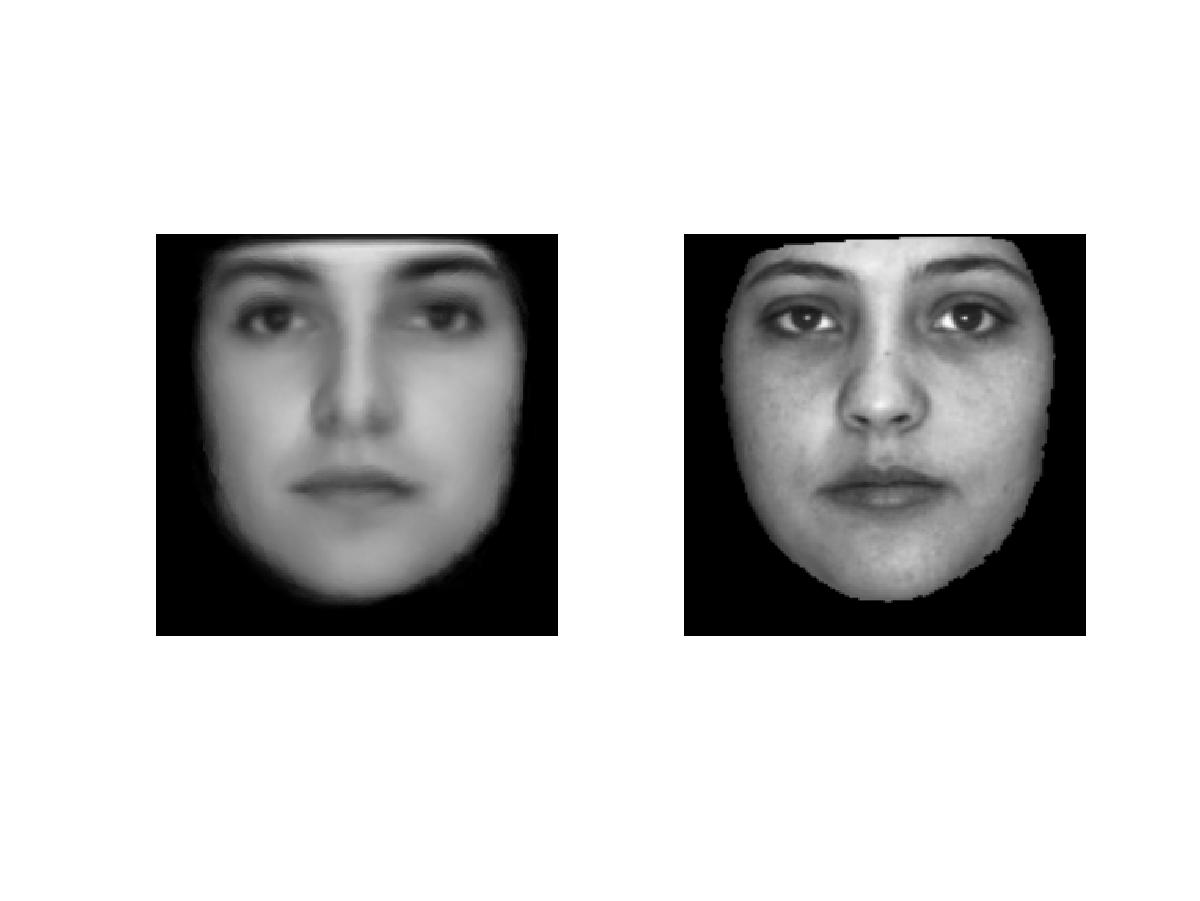
\includegraphics[scale=0.18]{c_rec_face_wf14.jpg}
  \caption{Reconstructed Faces}
\end{figure}


The reconstruction error shows as Figure.14. As we can see, the reconstruction error is smaller than that without wrapping stage. 
\begin{figure}[H]
  \centering
  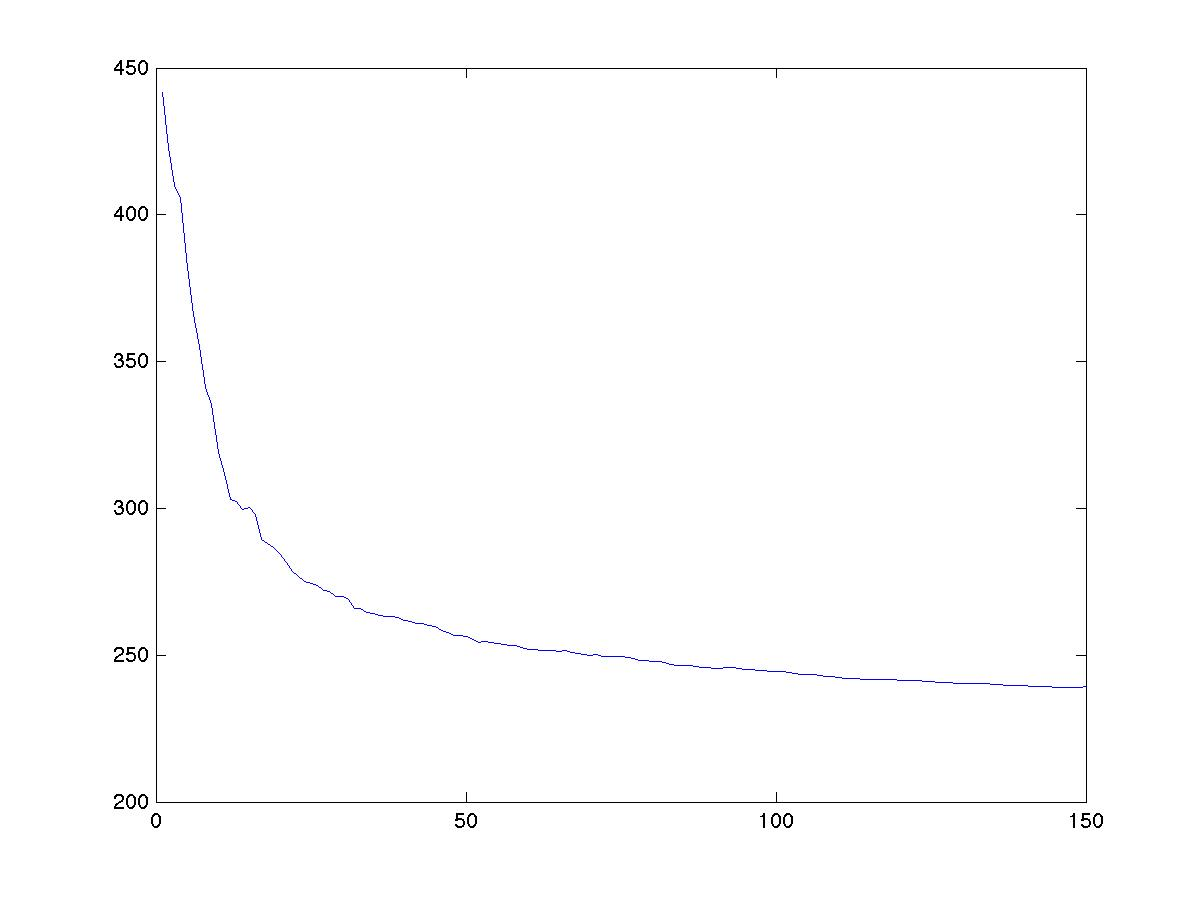
\includegraphics[scale=0.25]{rc_wf_error.jpg}
  \caption{Reconstruct Error}
\end{figure}

\item
Each axis has its own unit, that is, the square-root of its eigen-value. I choose normal distribution to get 20 random faces as following.
\begin{figure}[H]
  \centering
  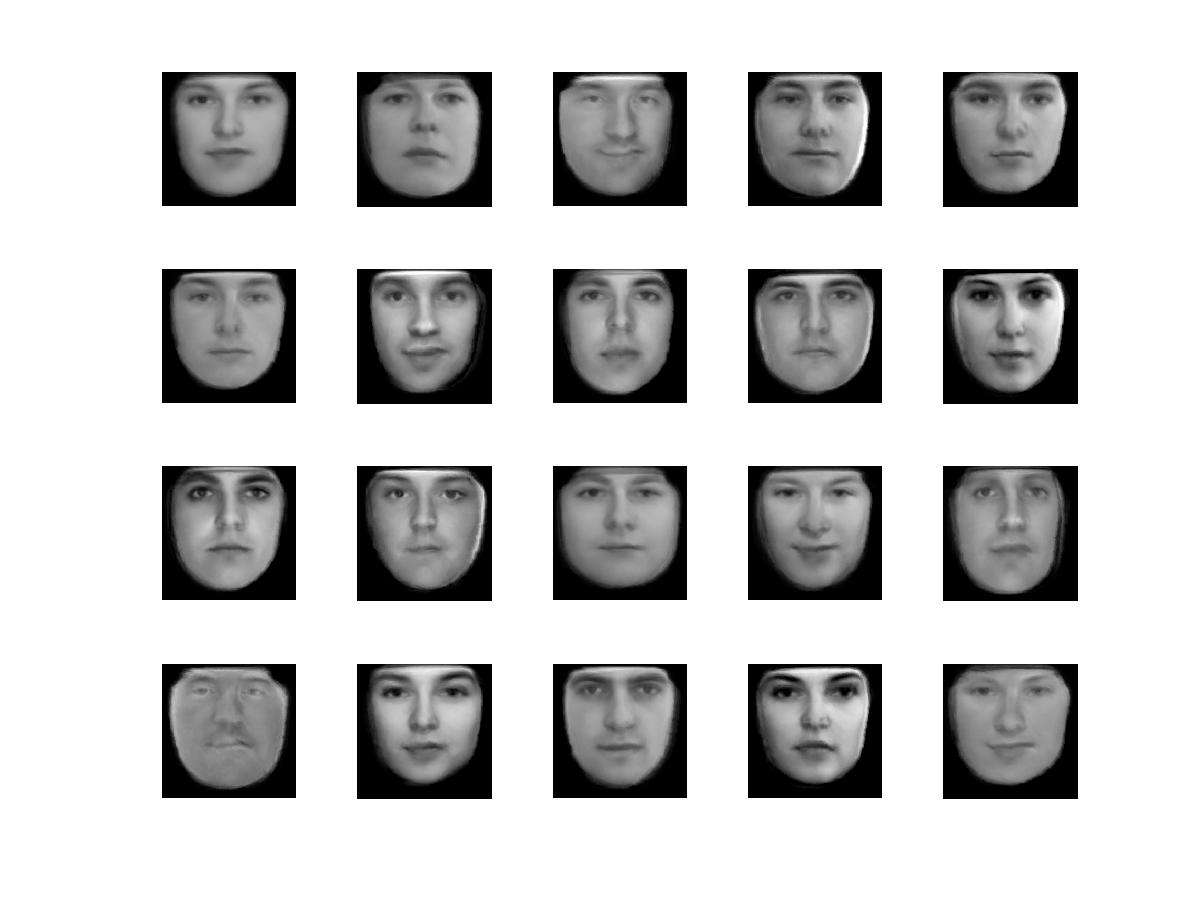
\includegraphics[scale=0.25]{d_random_face.jpg}
  \caption{Random Faces}
\end{figure}

\section{Part 2}
\item 
We get the first 10 faces in male and first 10 faces in female as test sets, the remaining faces will be used as training sets. However, the scatter matrix is very high dimensional, we have two way to solve Fisher in such high dimensional. 
\begin{enumerate}
\item
The first way is to follow instruction in \url{http://www.stat.ucla.edu/~sczhu/Courses/UCLA/Stat_231/Project_I/compute\%20the\%20Fisher\%20Face.pdf}. The result of this method is showed in Figure.16.
\begin{figure}[H]
  \centering
  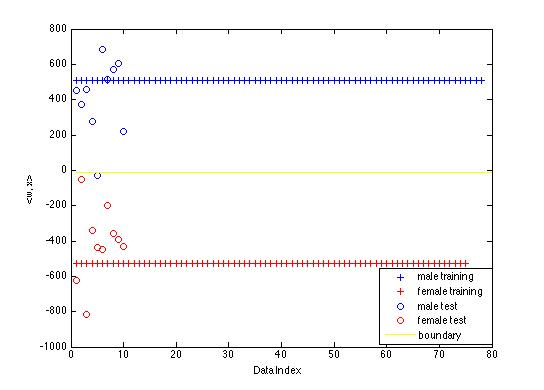
\includegraphics[scale=0.5]{a_fisher_direct.jpg}
  \caption{Fisher Result}
\end{figure}
As we can see, all test sets except one male face are correct, which means that we have about $\frac{19}{20}$ correct rate.\\
We find an interesting phenomenon where all male training sets projected into the same value, and all female training sets projected into another same value as well. How did this happen? The idea of Fisher is to project a higher dimension data into one dimension which is better for discriminating, and we can write down the projection equation $D' * w' = b$ where $D$ is data set where each column is an example and $w$ is projection vector. Since the number of datasets is far smaller than the number of features, then no matter what $b$ is, we can find the $w$ which satisfies $D' * w' = b$. For fisher algorithm, the best situation is all the dataset belonging in one class should be project into the same value, and we actually can find such $w$. Therefore, we can see such phenomenon. 
\item
Second idea is to compute the Fisher over reduced dimensions by PCA. Figure.16 shows the results which reduced dimension into 10. Figure.17 shows the results which reduced dimension into 50.

\begin{figure}[H]
  \centering
  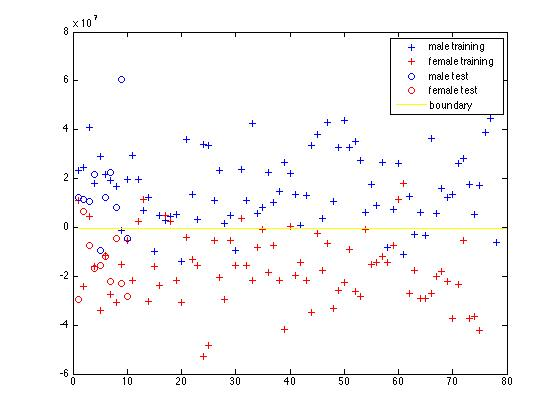
\includegraphics[scale=0.5]{a_fisher_pca10.jpg}
  \caption{Fisher Result within 10-dimension by PCA}
\end{figure}
\begin{figure}[H]
  \centering
  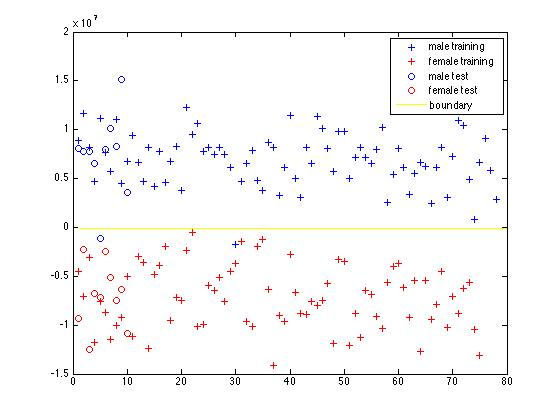
\includegraphics[scale=0.5]{a_fisher_pca50.jpg}
  \caption{Fisher Result within 50-dimension by PCA}
\end{figure}

\end{enumerate}

\item
In this case, I used PCA to reduced both feature space. Figure.18 shows the results which reduced dimension into 10. Figure.18 shows the results which reduced dimension into 50. X-axis denotes the projection value for Fisher of face image. Y-axis denotes the projection value for Fisher of Key point. Yellow line denotes the boundary.
\begin{figure}[H]
  \centering
  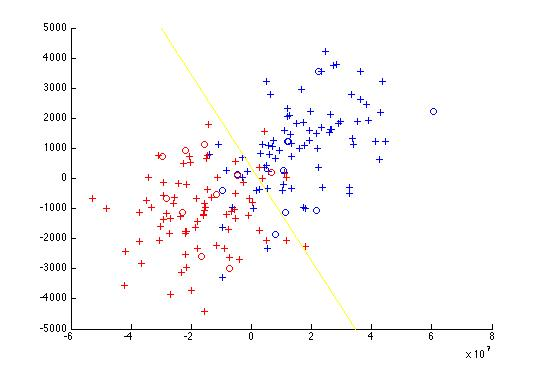
\includegraphics[scale=0.5]{b_fisher_pca10.jpg}
  \caption{2D-feature space: Fisher Result within 10-dimension by PCA}
\end{figure}
\begin{figure}[H]
  \centering
  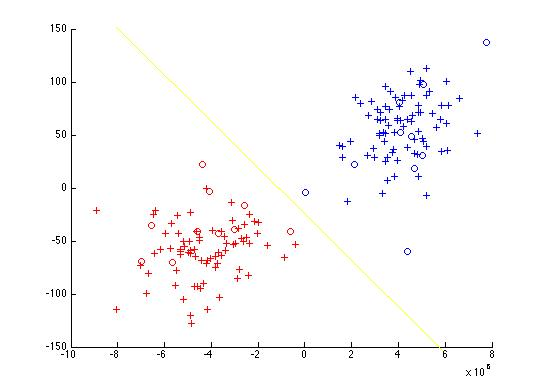
\includegraphics[scale=0.5]{b_fisher_pca50.jpg}
  \caption{2D-feature space: Fisher Result within 50-dimension by PCA}
\end{figure}
\end{enumerate}
With reducing dimension into smaller dimensional space, we are losing lots of information, so in 10-dimension space, we get bad performance which shows in Figure.18. However, when we increase the dimension of the space of PCA, we get a better results. As we can see in Figure.18, the correct rate is 100\%.



\end{document}
